%!TEX program = xelatex
\documentclass[a4paper,12pt]{report}
\usepackage{indentfirst} 
\usepackage{ctex}
%\usepackage{xeCJK}
\usepackage{times}
\usepackage{graphicx,float}
\usepackage{subcaption}
\usepackage{setspace}
\usepackage{fancyhdr}
% \usepackage{graphicx}
\usepackage{wrapfig}
\usepackage{array}
\usepackage{fontspec,xunicode,xltxtra}
\usepackage{titlesec}
\usepackage{titletoc}
\usepackage[titletoc]{appendix}
\usepackage[top=30mm,bottom=30mm,left=20mm,right=20mm]{geometry}
\usepackage{cite}
\usepackage{listings}
\usepackage[framed,numbered,autolinebreaks,useliterate]{mcode} % 插入代码
\XeTeXlinebreaklocale "zh"
\XeTeXlinebreakskip = 0pt plus 1pt minus 0.1pt

%---------------------------------------------------------------------
%	页眉页脚设置
%---------------------------------------------------------------------
\fancypagestyle{plain}{
	\pagestyle{fancy}      %改变章节首页页眉
}

\pagestyle{fancy}
\lhead{\kaishu~``计算机网络''实验报告~}
\rhead{\kaishu~~实验2:IP 与 ICMP 分析}
\cfoot{\thepage}

%---------------------------------------------------------------------
%	章节标题设置
%---------------------------------------------------------------------
\titleformat{\chapter}{\centering\zihao{-1}\heiti}{实验\chinese{chapter}}{1em}{}
\titlespacing{\chapter}{0pt}{*0}{*6}

%---------------------------------------------------------------------
%	摘要标题设置
%---------------------------------------------------------------------
\renewcommand{\abstractname}{\zihao{-3} 摘\quad 要}

%---------------------------------------------------------------------
%	参考文献设置
%---------------------------------------------------------------------
\renewcommand{\bibname}{\zihao{2}{\hspace{\fill}参\hspace{0.5em}考\hspace{0.5em}文\hspace{0.5em}献\hspace{\fill}}}

%---------------------------------------------------------------------
%	引用文献设置为上标
%---------------------------------------------------------------------
\makeatletter
\def\@cite#1#2{\textsuperscript{[{#1\if@tempswa , #2\fi}]}}
\makeatother

%---------------------------------------------------------------------
%	目录页设置
%---------------------------------------------------------------------
\titlecontents{chapter}[0em]{\songti\zihao{-4}}{\thecontentslabel\ }{}
{\hspace{.5em}\titlerule*[4pt]{$\cdot$}\contentspage}
\titlecontents{section}[2em]{\vspace{0.1\baselineskip}\songti\zihao{-4}}{\thecontentslabel\ }{}
{\hspace{.5em}\titlerule*[4pt]{$\cdot$}\contentspage}
\titlecontents{subsection}[4em]{\vspace{0.1\baselineskip}\songti\zihao{-4}}{\thecontentslabel\ }{}
{\hspace{.5em}\titlerule*[4pt]{$\cdot$}\contentspage}

\renewcommand\thesection{\arabic{section}}
\renewcommand\thesubsection{\arabic{section}.\arabic{subsection}}
\setcounter{tocdepth}{3}
\setcounter{secnumdepth}{3}
\begin{document}
%---------------------------------------------------------------------
%	封面设置
%---------------------------------------------------------------------
\begin{titlepage}
	\begin{center}
		
    
\includegraphics[width=1.0\textwidth]{figure//nankai.jpg}\\
    % \vspace{10mm}
    % \textbf{\zihao{2}\kaishu{软件学院}}\\[0.8cm]
    \vspace{50mm}
    \textbf{\zihao{1}\heiti{ 《计算机网络》实验报告}}\\[1cm]
    \textbf{\zihao{2}\heiti{ (2022\textasciitilde2023学年第一学期)}}\\[1cm]
    % \textbf{\zihao{3}\heiti{ 实验1: Wireshark 软件使用与ARP 协议分析}}\\[2cm]
	\vspace{\fill}
	
\setlength{\extrarowheight}{2mm}
{\songti\zihao{3}	
\begin{tabular}{rl}

	{\makebox[4\ccwd][s]{实验名称:}}& ~\kaishu IP 与 ICMP 分析\\
	{\makebox[4\ccwd][s]{学\qquad 院:}}& ~\kaishu 软件学院\\
		{\makebox[4\ccwd][s]{姓\qquad 名:}}& ~\kaishu 张怡桢\\

    {\makebox[4\ccwd][s]{学\qquad 号:}}& ~\kaishu 2013747 \\

	{\makebox[4\ccwd][s]{指导老师:}} & ~\kaishu 张圣林\\

\end{tabular}
 }\\[2cm]
\vspace{\fill}
\zihao{4}
%2021\textasciitilde 2022秋季学期\\
%使用\LaTeX 撰写于
    \today
	\end{center}	
\end{titlepage}


%---------------------------------------------------------------------
%  目录页
%---------------------------------------------------------------------
\tableofcontents % 生成目录

%---------------------------------------------------------------------
%  实验一
%---------------------------------------------------------------------
\chapter*{IP 与 ICMP 分析
}
\setcounter{page}{1}
\begin{spacing}{1.5}
\songti\zihao{-4}

%\section{分工情况}
 %\begin{itemize}
 %	\item 张三:
 %	\item 李四:
 %	\item 六六:
 %\end{itemize}
\section{实验目的}
IP 和 ICMP 协议是 TCP/IP 协议簇中的网络层协议,在网络寻址定位、数据分组转 发和路由选择等任务中发挥了重要作用。本实验要求熟练使用 Wireshark 软件,观察 IP 数据报的基本结构,分析数据报的分片;掌握基于 ICMP 协议的 ping 和 tracert 命令及 其工作原理。

\section{实验条件}
装有 Wireshark 软件的 PC 机一台,处于局域网环境。

\section{实验内容}
启动 Wireshark,捕捉网络命令执行过程中本机接受和发送的数据报。

1. 执行 ping 命令,观察 IP 数据报和 ICMP 询问报文的结构:通过 Wireshark 监视 器观察捕获流量中的 ICMP 询问报文和 IP 数据报的结构。注意比较 ICMP 请求 帧与回应帧,及其 IP 头部数据字段的异同。

2. 改变 ping 命令的参数,观察 IP 数据报分片:更改 ping 命令参数 MTU,使其发 出长报文以触发 IP 数据报分片,再观察 IP 数据报的结构变化。

3. 执行 Tracert 命令,观察 ICMP 差错报文的结构,并分析其工作原理:使用 Linux 操作系统提供的 tracert6 命令(或者 Windows 系统提供的 tracert 命令), 捕获和分析该命令所产生的 IP 数据报,特别注意相关的 ICMP 差错报文。结合 捕获的具体数据,画出命令执行过程中数据交互的示意图,掌握 tracert 的工作原理。

\section{实验过程}
\subsection{执行ping命令,观察IP数据报和ICMP询问报文结构}
本机(IP 为 10.22.7.88)启动 Wireshark 软件,选择要监听的网络接口:WiFi:en0;然后在终端发起网络命令:ping baidu.com。
\begin{figure}[htb!]
  \centering
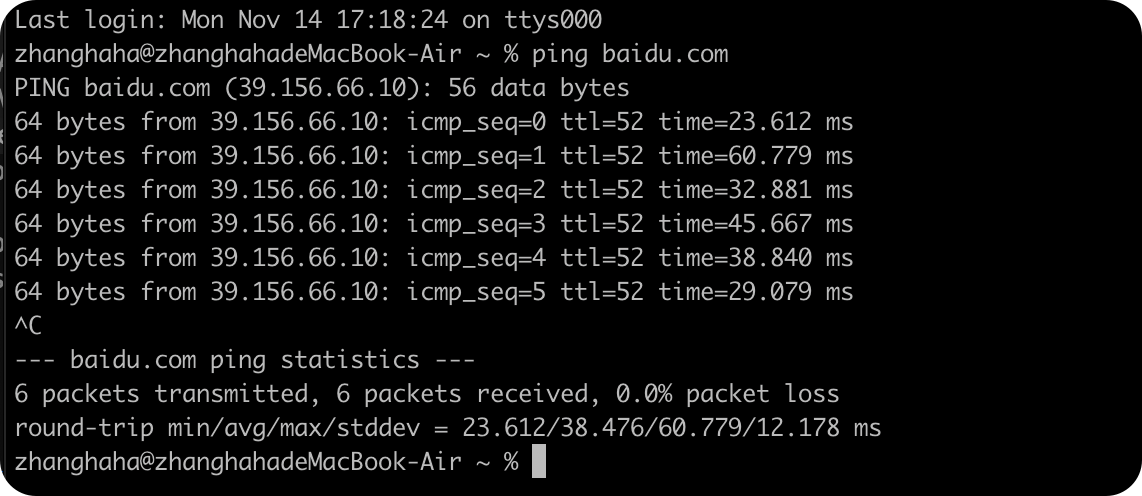
\includegraphics[width=10cm]{figure/pingbaidu.png}
\caption{ping baidu.com}
\label{pic1}
\end{figure}

在 Wireshark 监视器中设置过滤条件。设置过滤条件为 icmp,则显 示出所捕获的 ICMP 数据包。
\begin{figure}[htb!]
  \centering
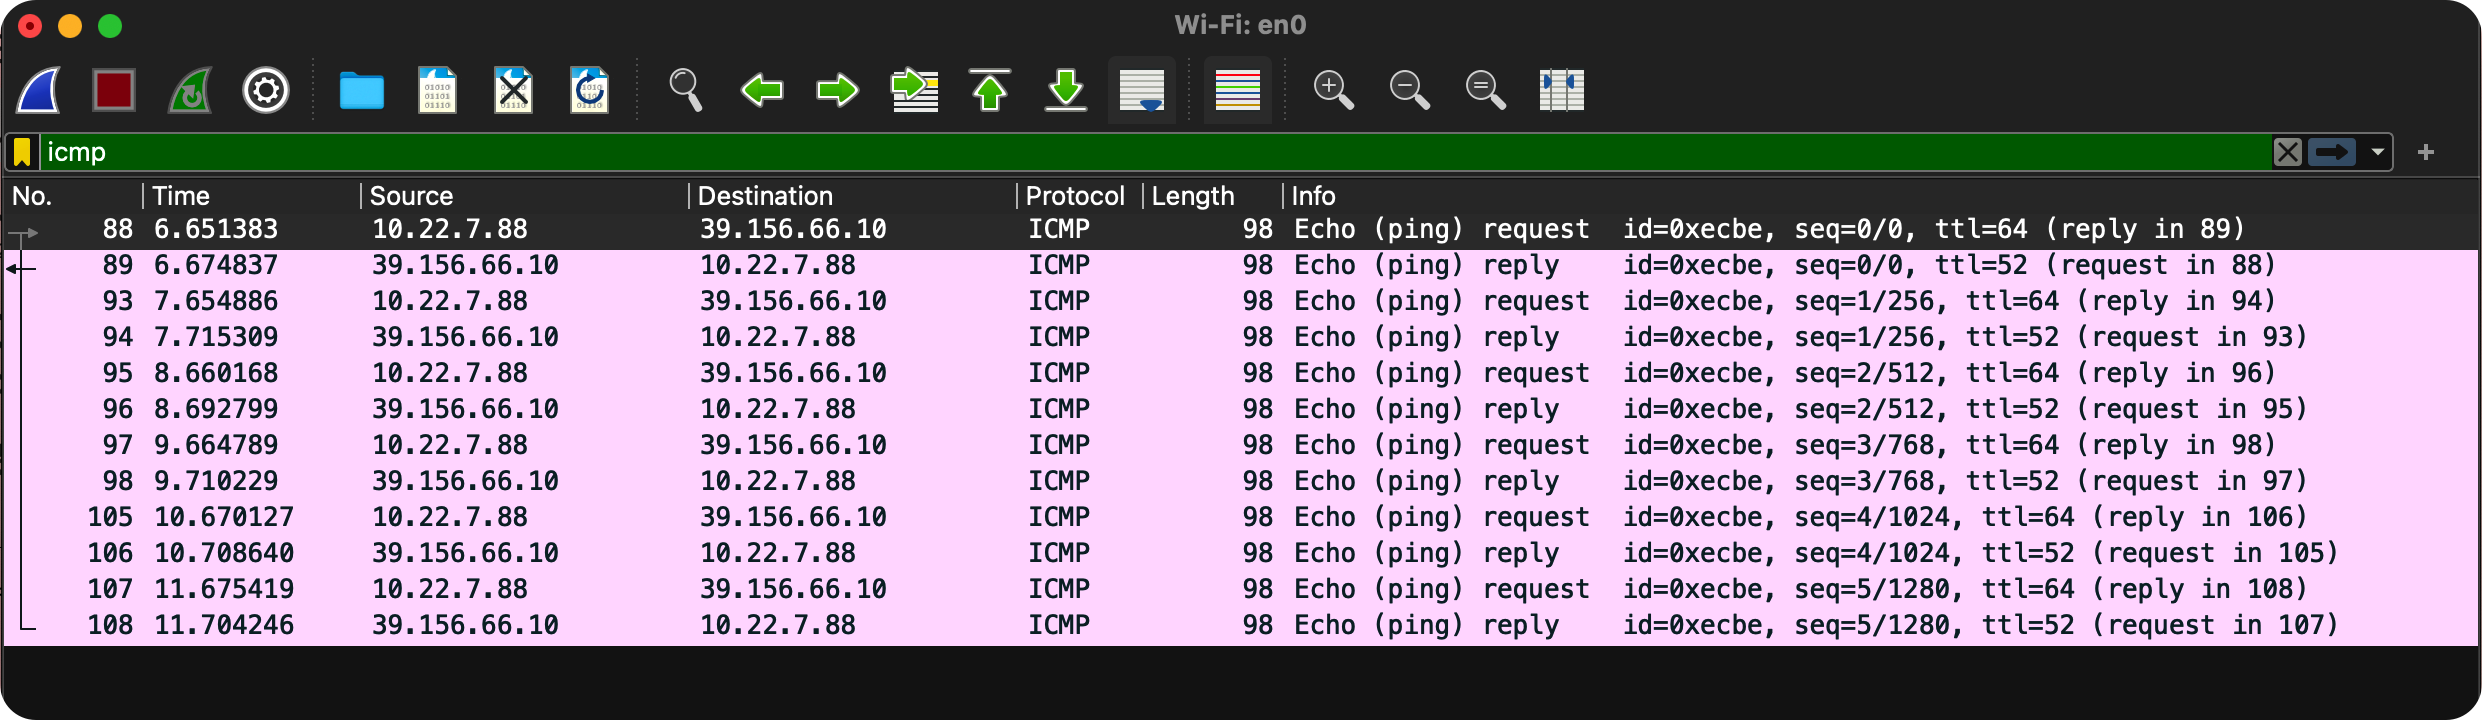
\includegraphics[width=12cm]{figure/pingbaidu_wireshark.png}
\caption{wireshark 抓取icmp}
\label{pic2}
\end{figure}

\subsubsection{IP数据报结构}
点击 Internet Protocol Version 4 展开,查看 IP 数据报,特别观察 IP 数据报的首部字段及其内容。
\begin{figure}[htb!]
  \centering
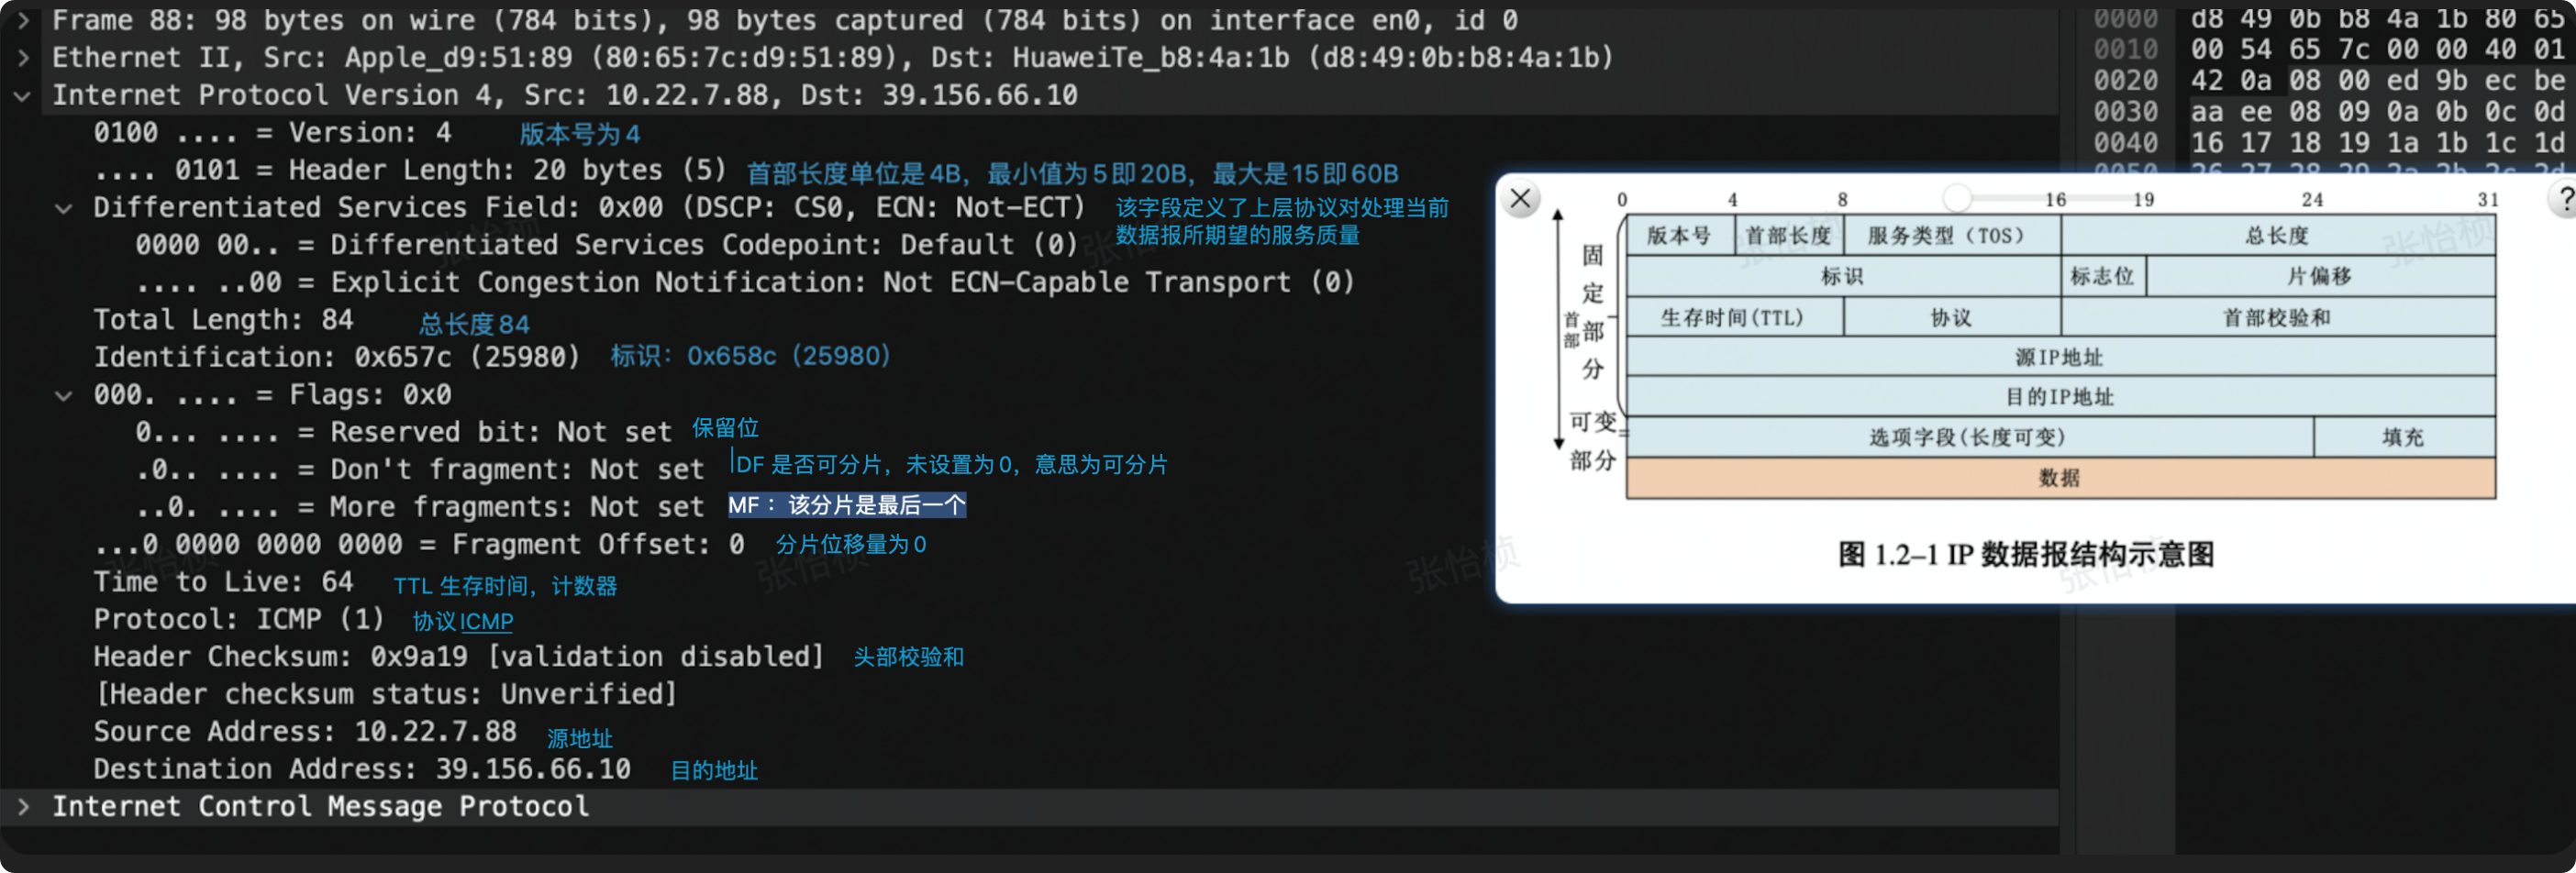
\includegraphics[width=14cm]{figure/ipv4.png}
\caption{IP数据报结构分析}
\label{pic3}
\end{figure}


1. 版本(4 位):该字段定义 IP 协议版本,该例的IP协议版本号为4。

2. 首部长度(4 位):该字段定义数据报协议头长度,表示协议首部具有 32 位字长 的数量,最小值为 5,最大值为 15。该例中的首部长度为 5,该字段单位为4B,即 20 字节。

3. 服务(8 位):该字段定义上层协议对处理当前数据报所期望的服务质量,并对 数据报按照重要性级别进行分配。前 3 位为优先位,后面 4 位为服务类型,最后 1 位没有定义。这 8 位可用于分配优先级、延迟、吞吐量以及可靠性。

4. 总长度(16 位):该字段定义整个 IP 数据报的字节长度,包括协议首部和数据, 其最大值为 65535 字节。该字段单位为1B,该例中的总长度为 84字节。

5. 标识(16 位):用于唯一标识主机发送的每一份数据报。通常每发送一个报文,它的值加一。当IP报文长度超过传输网络的MTU(最大传输单元)时必须分片,这个标识字段的值被复制到所有数据分片的标识字段中,使得这些分片在达到最终目的地时可以依照标识字段的内容重新组成原先的数据。该例中的标识字段为0x657c。

6. 标记(3 位):该字段由 3 位字段构成,其中最低位(MF)控制分片:若存在下 一个分片则值为 1;否则置 0 代表该分片是最后一个。图中该字段标识为0,表示该分片是最后一个。
中间位(DF)指出数据报 是否可进行分片,若置 1 则不允许该数据报进行分片,图中该位为 0,表示该数据报可进行分片。
第三位即最高位保留不 使用,值为 0。图中该字段标识为0。

7. 分片偏移(13 位):该字段指出数据分片在源数据报中的相对位置,以 8 字节为 长度单位。该例中的分片偏移为 0。

8. 生存时间(8 位):IP报文所允许通过的路由器的最大数量。每经过一个路由器,TTL减1,当为0时,路由器将该数据报丢弃。TTL字段是由发送端初始设置一个8 bit字段。该例发送ICMP回显请求时TTL设置的值为64。

9. 协议:指出IP报文携带的数据使用的是那种协议,以便目的主机的IP层能知道要将数据报上交到哪个进程(不同的协议有专门不同的进程处理)。和端口号类似,此处采用协议号,TCP的协议号为6,UDP的协议号为17。ICMP的协议号为1,IGMP的协议号为2。该例中携带数据使用的是ICMP协议,协议号为1。

10. 首部校验和:该字段帮助确保 IP 协议头的正确性。计算过程是先将校验和字段置为 0,然后将整个头部每 16 位划分为一部分,并将各部分相加,其计算结果取反码,填入校验和字段中。可以看到该例中的首部校验和为0x9a19,且未被验证过。

11. 源地址和目的地址:均为32位,分别表示源主机和目标主机的IP地址。

Source Address: 10.22.7.88

Destination Address: 39.156.66.10

\subsubsection{ICMP Echo 回显报文结构}
\begin{figure}[htb!]
  \centering
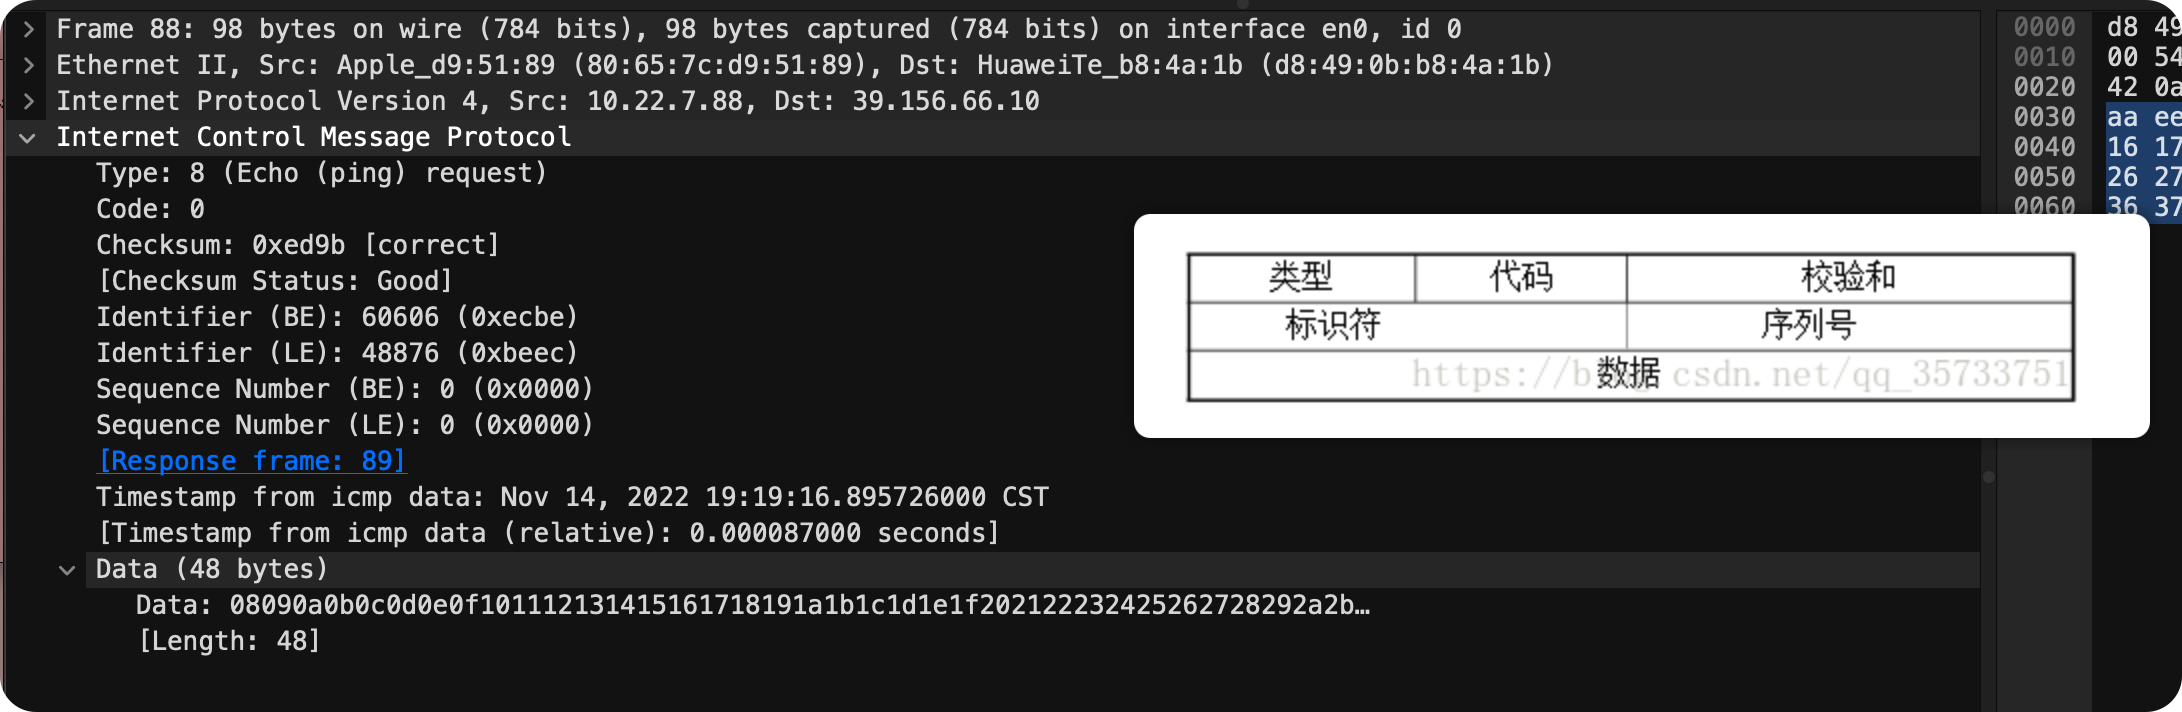
\includegraphics[width=12cm]{figure/echo_request.png}
  \caption{ICMP Echo request 回显报文结构}
  \label{fig:echo_request}
\end{figure}
\begin{figure}[htb!]
  \centering
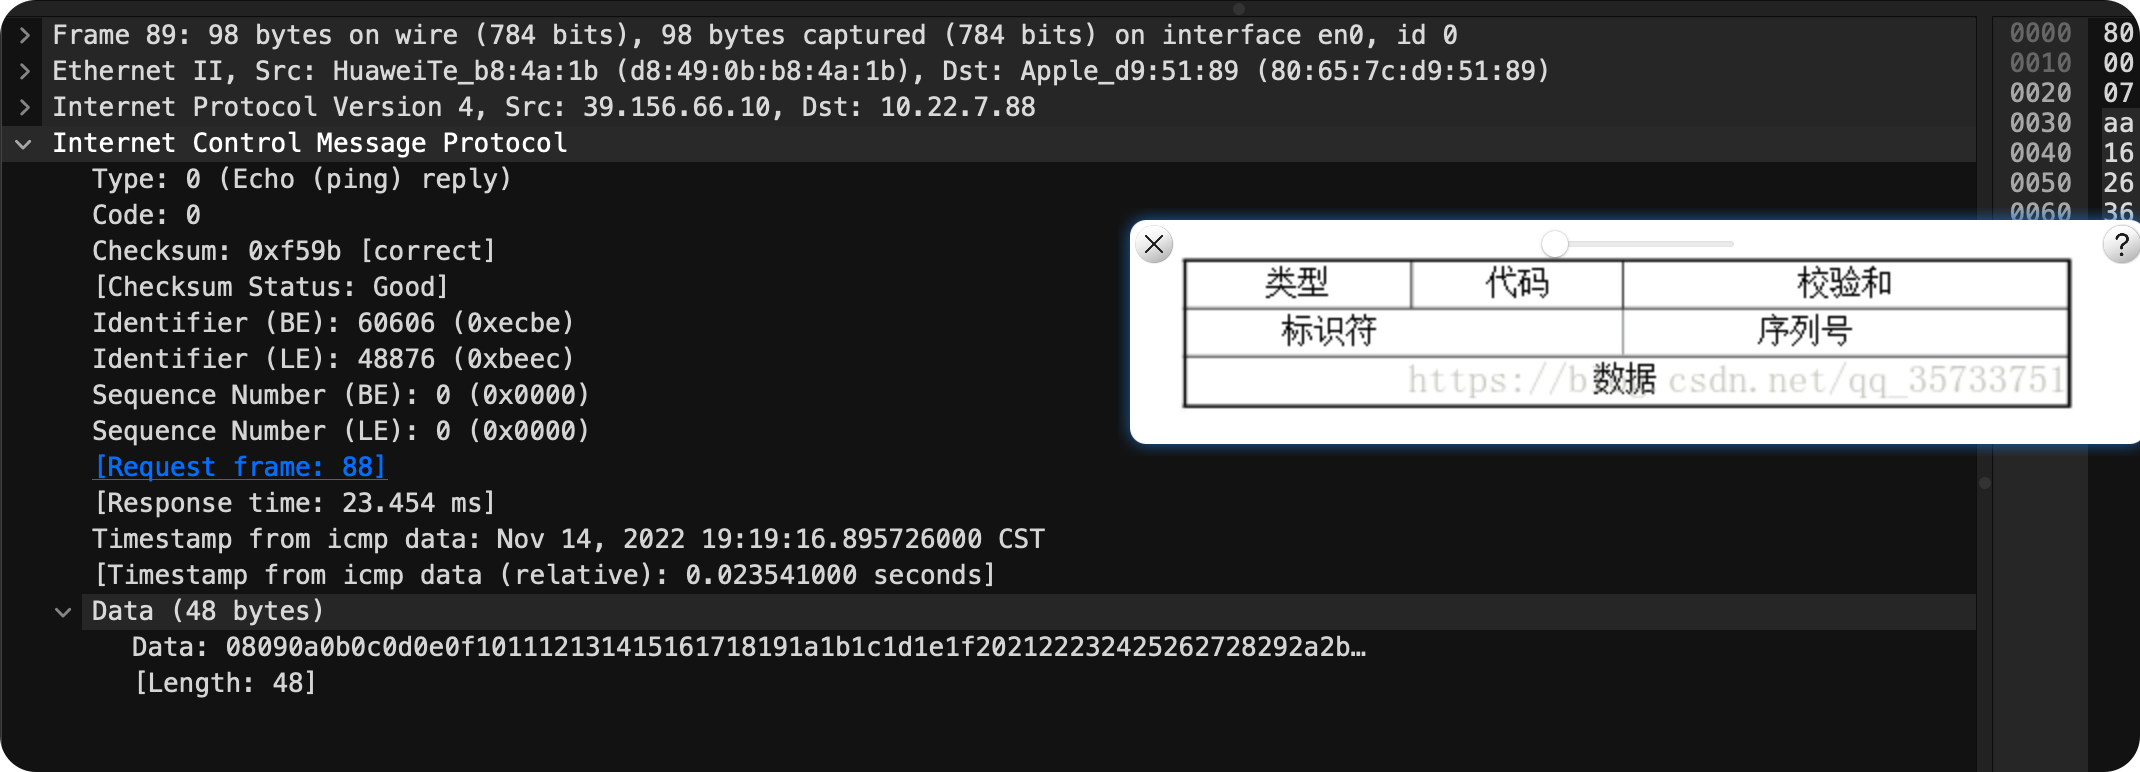
\includegraphics[width=12cm]{figure/echo_reply.png}
  \caption{ICMP Echo reply 回显报文结构}
  \label{fig:echo_reply}
\end{figure}

1. Type:该字段有1个字节,表示特定类型的ICMP报文。

2. Code:该字段有1个字节,进一步细分ICMP的类型。
在图 \ref{fig:echo_request} 中,Type的值为 8,Code 的值为0,表示该ICMP询问报文的种类为回显请求报文。

在图 \ref{fig:echo_reply}中,Type的值为 0,Code 的值为0,表示该ICMP应答报文的种类为回显应答报文。

具体的Type与Code的对应关系可以参考图 \ref{fig:TC}。

\begin{figure}[htb!]
  \centering
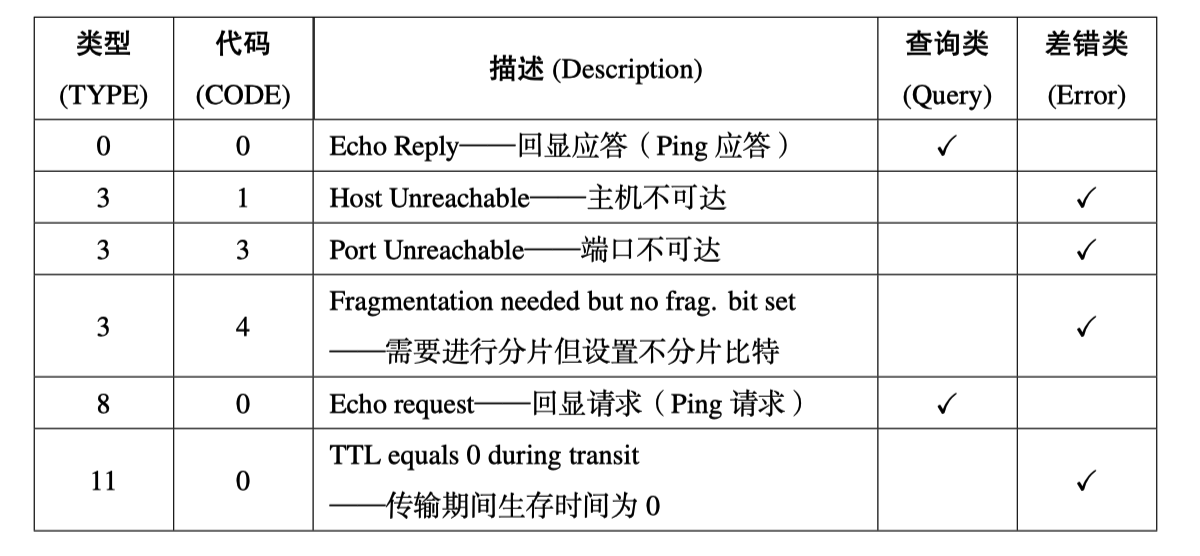
\includegraphics[width=12cm]{figure/TC.png}
  \caption{Type与Code的对应关系}
  \label{fig:TC}
\end{figure}

ICMP报文的类型可以分为ICMP差错报文和ICMP询问报文两种。ICMP差错报告报文主要有终点不可达、源站抑制、超时、参数问题和路由重定向5种。ICMP询问报文有回送请求和应答、时间戳请求和应答、地址掩码请求和应答以及路由器询问和通告4种。

3. Checksum:该字段有2个字节,表示校验和。由 ICMP 报头和数据部分计算得来的,用于检查错误的数据。上图两个ICMP询问报文的状态正常,没有错误。

4. Identifier标识符:该字段有 2 个字节,用于匹配 Request/Reply 的标识符。

5. Seq Num序列号:该字段有 2 个字节,用于匹配 Request/Reply 的序列号。

6. Data: 数据载荷。

7. 额外信息:frame数。
Echo Request中【Resonse frame:89】,表示这是第89帧。
Echo Reply中【Requst frame:88】,表示这是第88帧。
对于Echo Reply中还记载了【Respone time:23.454 ms】,表示回显时间为23.454 ms。

8. 额外信息:时间戳。
对于request报文,该字段存放发送时间戳;对于reply报文,该字段存放接收时间戳。



\subsection{改变ping命令参数,观察IP数据报分片}
清空 Wireshark 监控器,重新发起网络命令:ping IP 地址/域名–l length,
并解释对比前后两次执行 ping 命令的结果。
其中,-l length 确定 echo 数据报的长度为 length,其默认值为 32 字节,且小于 65,527 字节。

在图 \ref{pic:pc} 中,使用zhh去ping PC3,多次改变length 的大小( 1000 字节、2000 字节和 4000 字节)。ping的结果如\ref{pic:pingl}所示,全部都ping成功了。

\begin{figure}[htb!]
  \centering
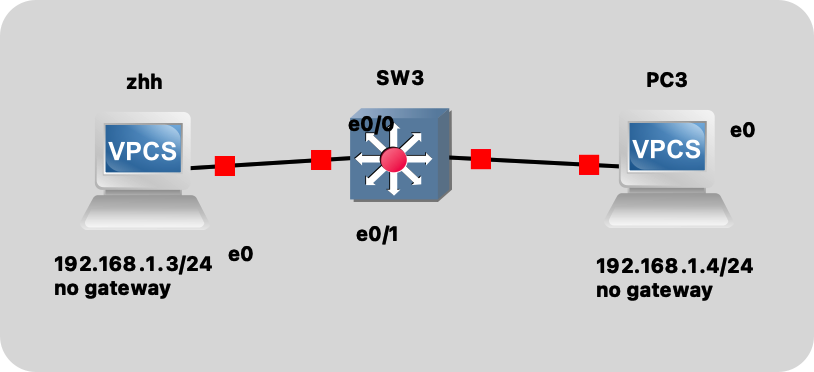
\includegraphics[width=8cm]{figure/pctopc.png}
\caption{网络拓扑图}
\label{pic:pc}
\end{figure}

\begin{figure}[htb!]
  \centering
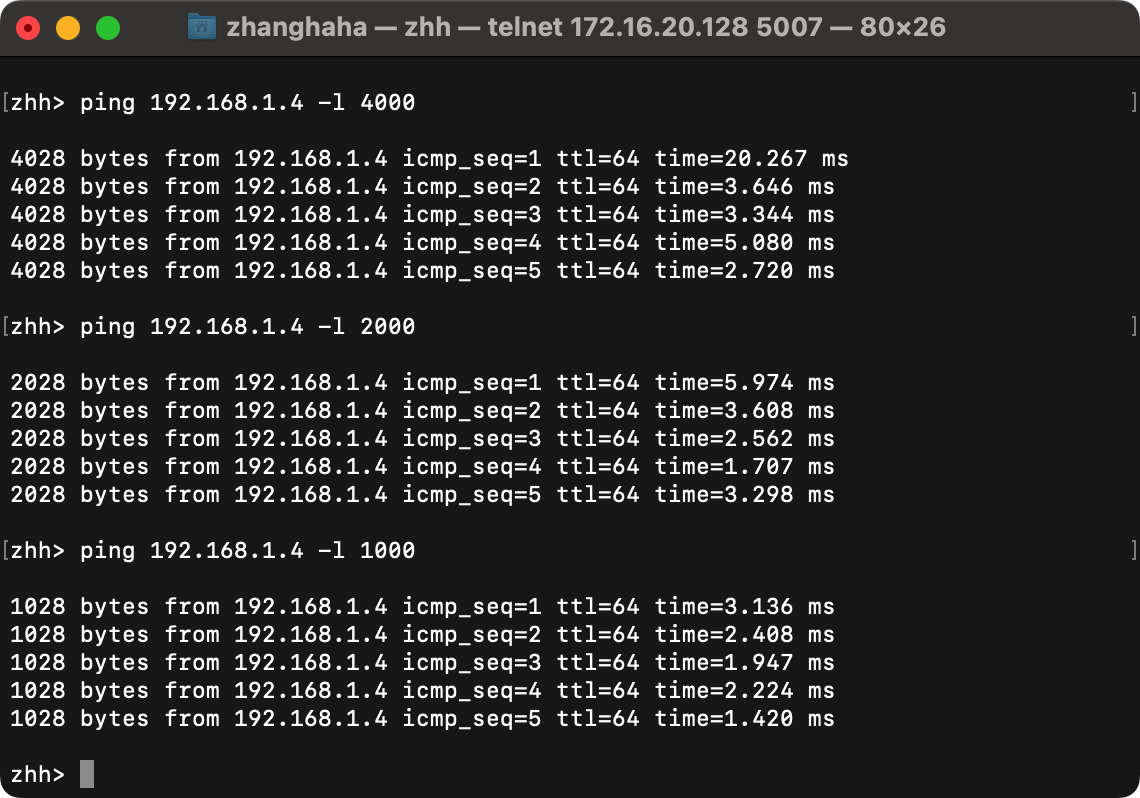
\includegraphics[width=10cm]{figure/pingl.png}
\caption{网络拓扑图}
\label{pic:pingl}
\end{figure}


\subsubsection{观察 IP 数据报何时会分片?} 


如下图为使用wireshark抓取的不同长度的报文,其中,图\ref{pic:1000}为长度为1000字节的报文,图\ref{pic:2000}为长度为2000字节的报文,图\ref{pic:4000}为长度为4000字节的报文。

可以看到,当长度为1000字节时,IP数据报没有分片,当长度为2000字节时,IP数据报分片了,当长度为4000字节时,IP数据报分片了。


\subsubsection{请解释 IP 数据报分片的原因和具体情况。}

最大传输单元(MTU):指由IP包头和数据部分组成的IP数据报长度。

帧长度=以太网帧首部(14字节)+IP数据报长度(MTU)。

IP数据报长度=IP包头长度(20字节)+ICMP首部长度(8字节)+数据部分长度(\#length)。

以太网中, MTU 设置为 1500。所以ICMP负载长度最大值为

MTU(1500字节) - IP首部长度(20字节)-ICMP首部长度(8字节) = 1472 字节

IP数据报的长度大于MTU(RFC标准定义以太网的默认MTU值为1500)时即ICMP(data)负载长度大于1472字节时,IP数据报会分片。

\subsubsection{请分析 IP 数据报分片的具体情况}

\paragraph{IPCM负载为1000}

如图\ref{pic:1000}与图 \ref{pic:1000data} 所示。

\begin{figure}[htb!]
  \centering
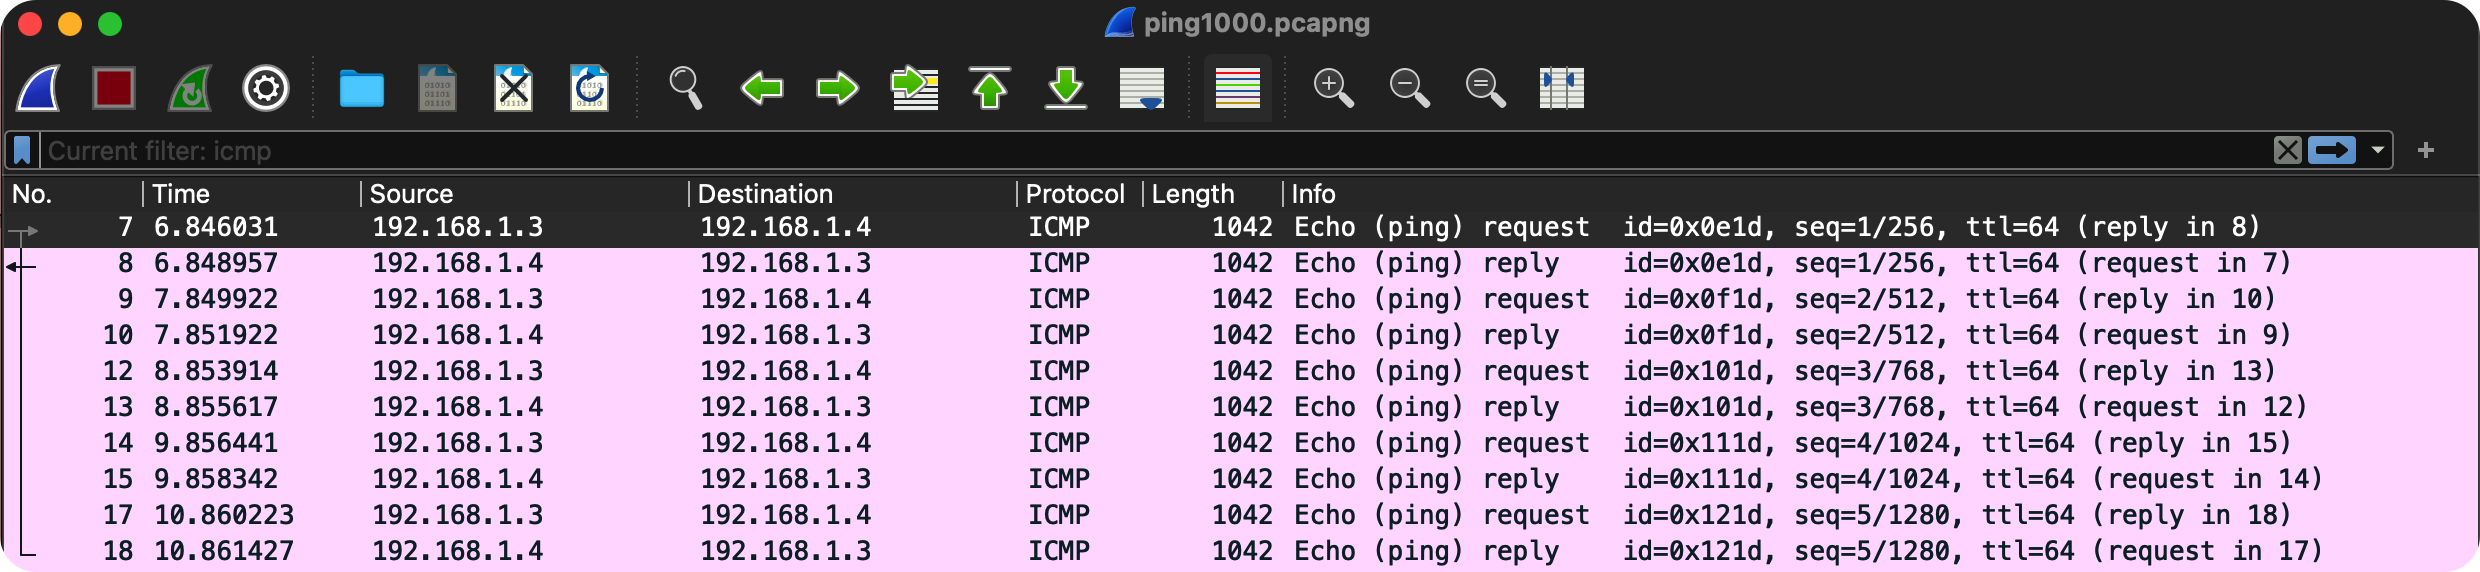
\includegraphics[width=10cm]{figure/ping1000.png}
\caption{length=1000}
\label{pic:1000}
\end{figure}


\begin{figure}[htb!]
  \centering
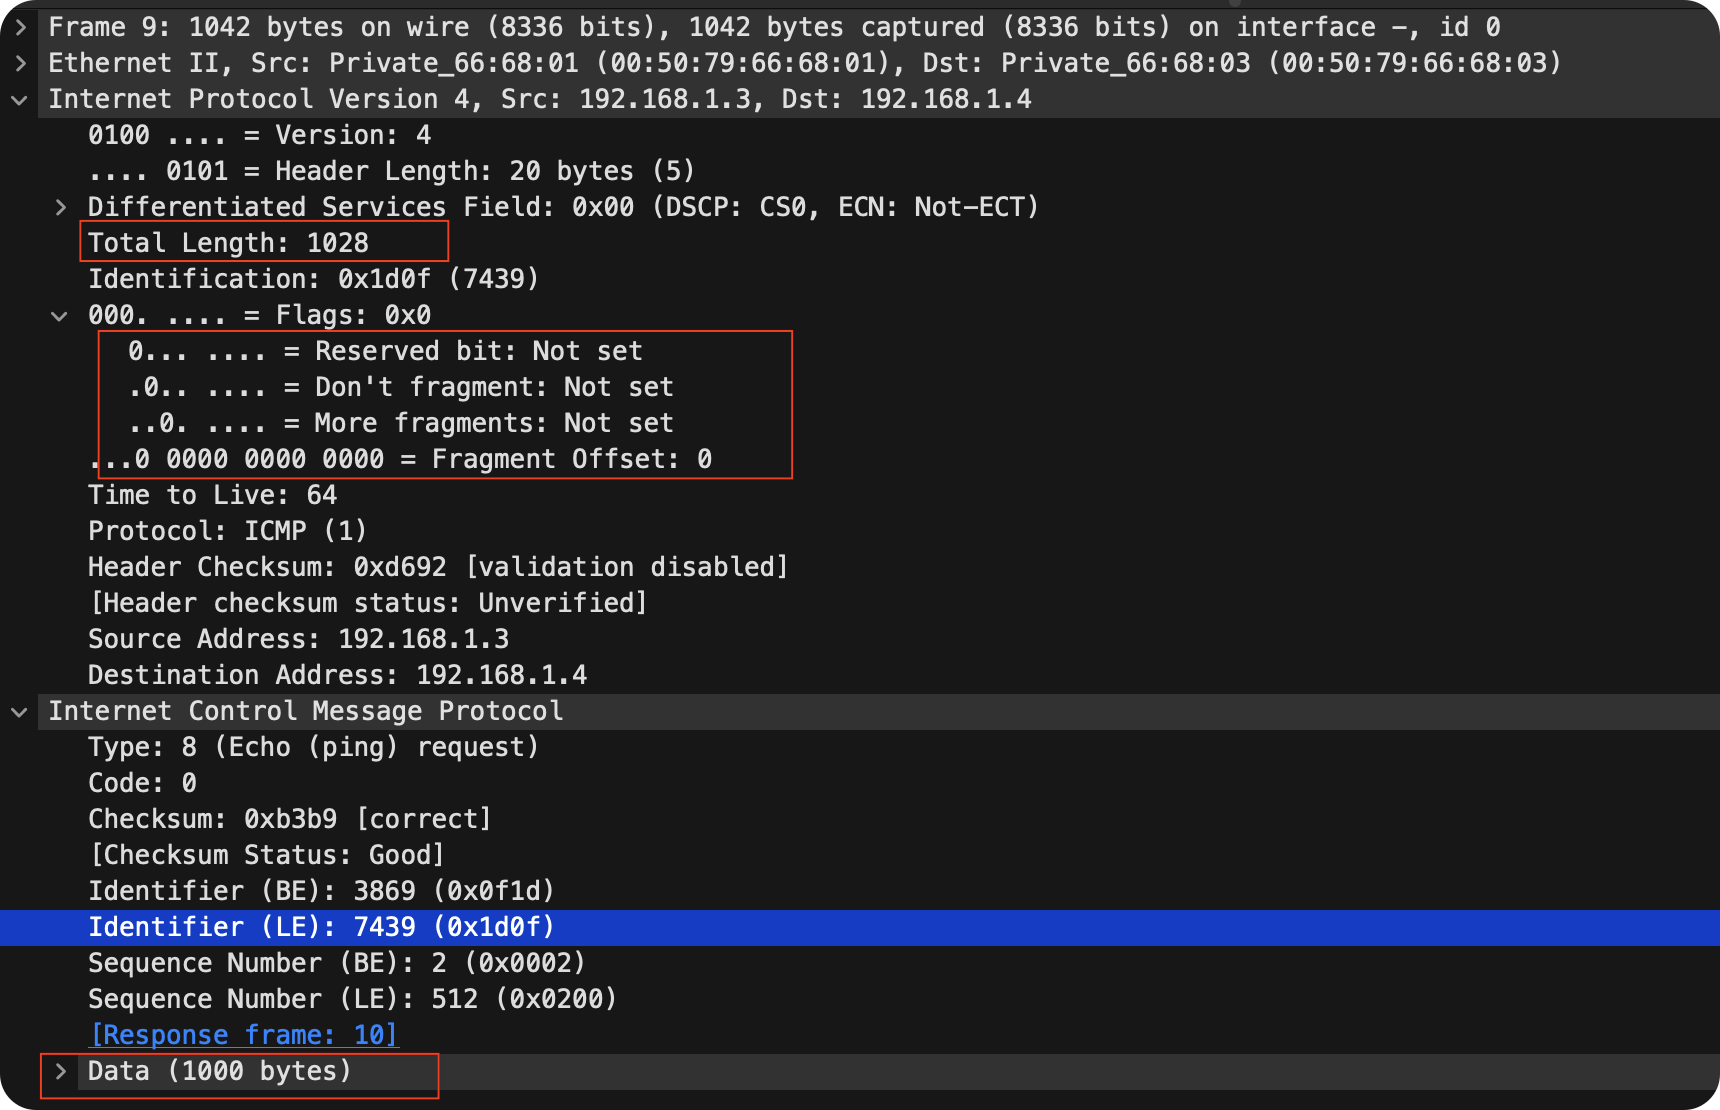
\includegraphics[width=10cm]{figure/ping1000_data.png}
\caption{length=1000 分析}
\label{pic:1000data}
\end{figure}


ICMP负载字节为1000时,小于改值,不分片,可以看到ICMP报文帧的长度为1042字节,其结构为

帧长度1042 = 以太网帧首部(14字节) + IP首部(20字节) + ICMP首部(8字节)+ ICMP 负载长度(1000字节)


\paragraph{IPCM负载为2000}

图\ref{pic:2000_ipv4} 是第一个ipv4数据包,图\ref{pic:2000_icmp} 是第二个icmp数据包

\begin{figure}[htb!]
  \centering
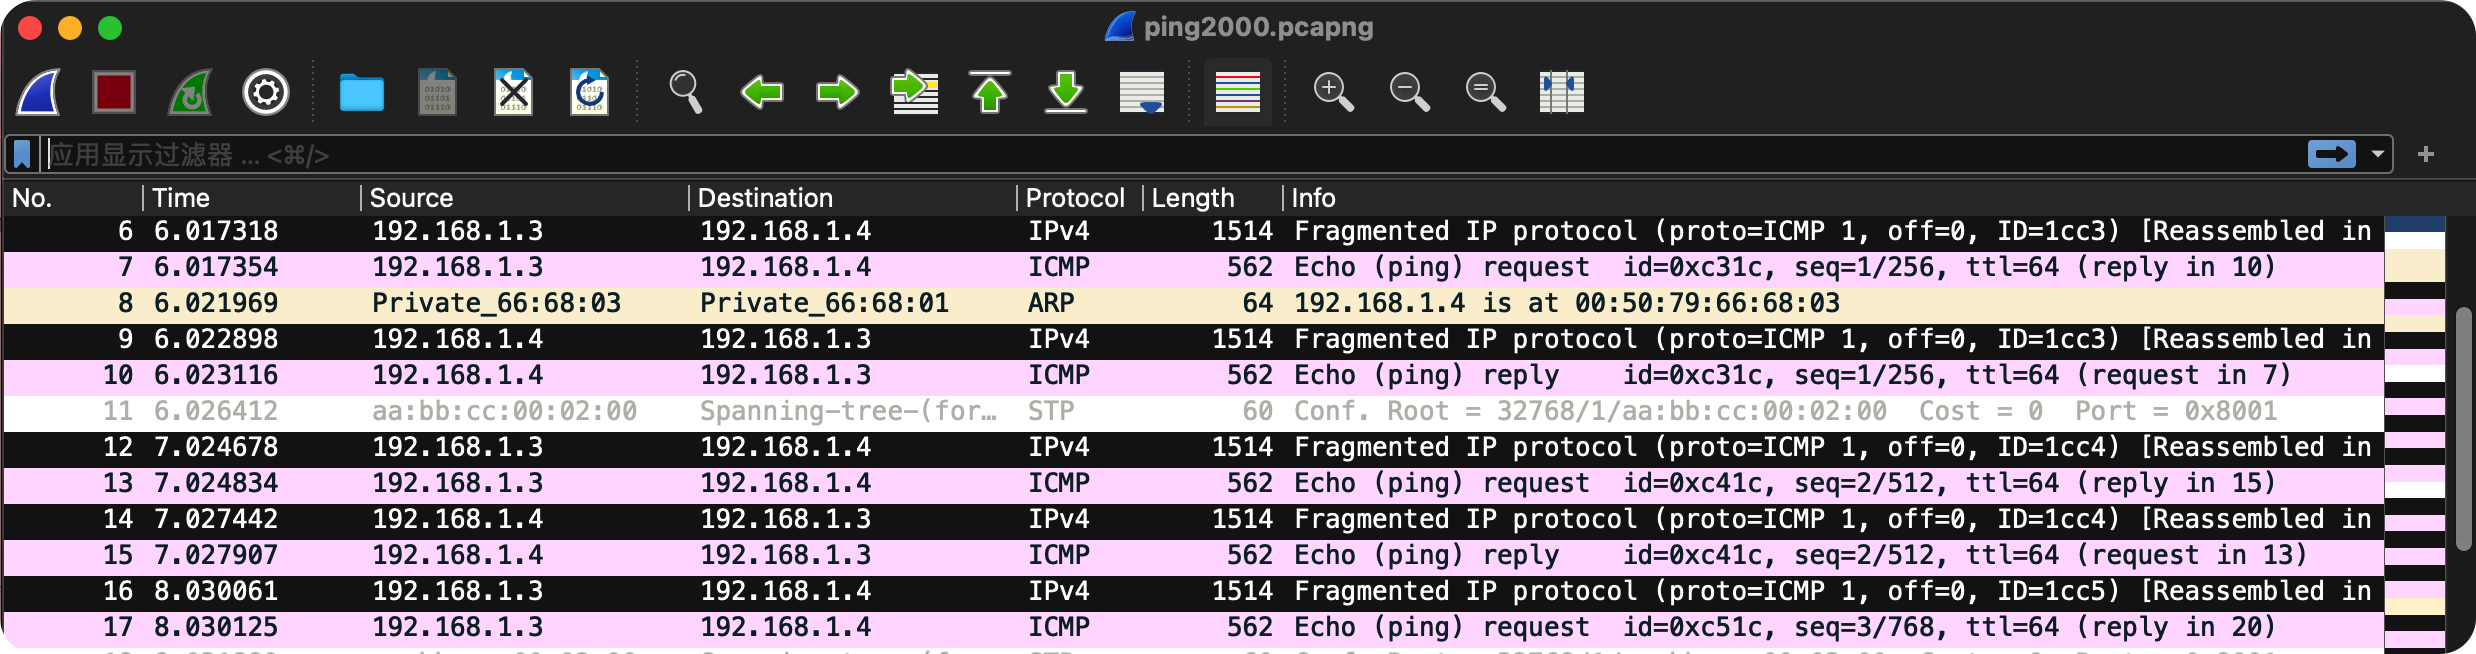
\includegraphics[width=10cm]{figure/ping2000.png}
\caption{length=2000}
\label{pic:2000}
\end{figure}


在图\ref{pic:2000_ipv4}中,MF位为1,DF位为0,说明该IP数据报是分片的,且不是最后一个分片。
其在ipv4层的标识为0x1cc3(7363),偏移量为0,说明该IP数据报是第一个分片。

作为Frame6的ipv4数据帧中,标识了蓝字【Reassembled IPv4 in frame 7】,说明该IP数据报将在frame 7 也就是下一个分片被重组。

\begin{figure}[htb!]
  \centering
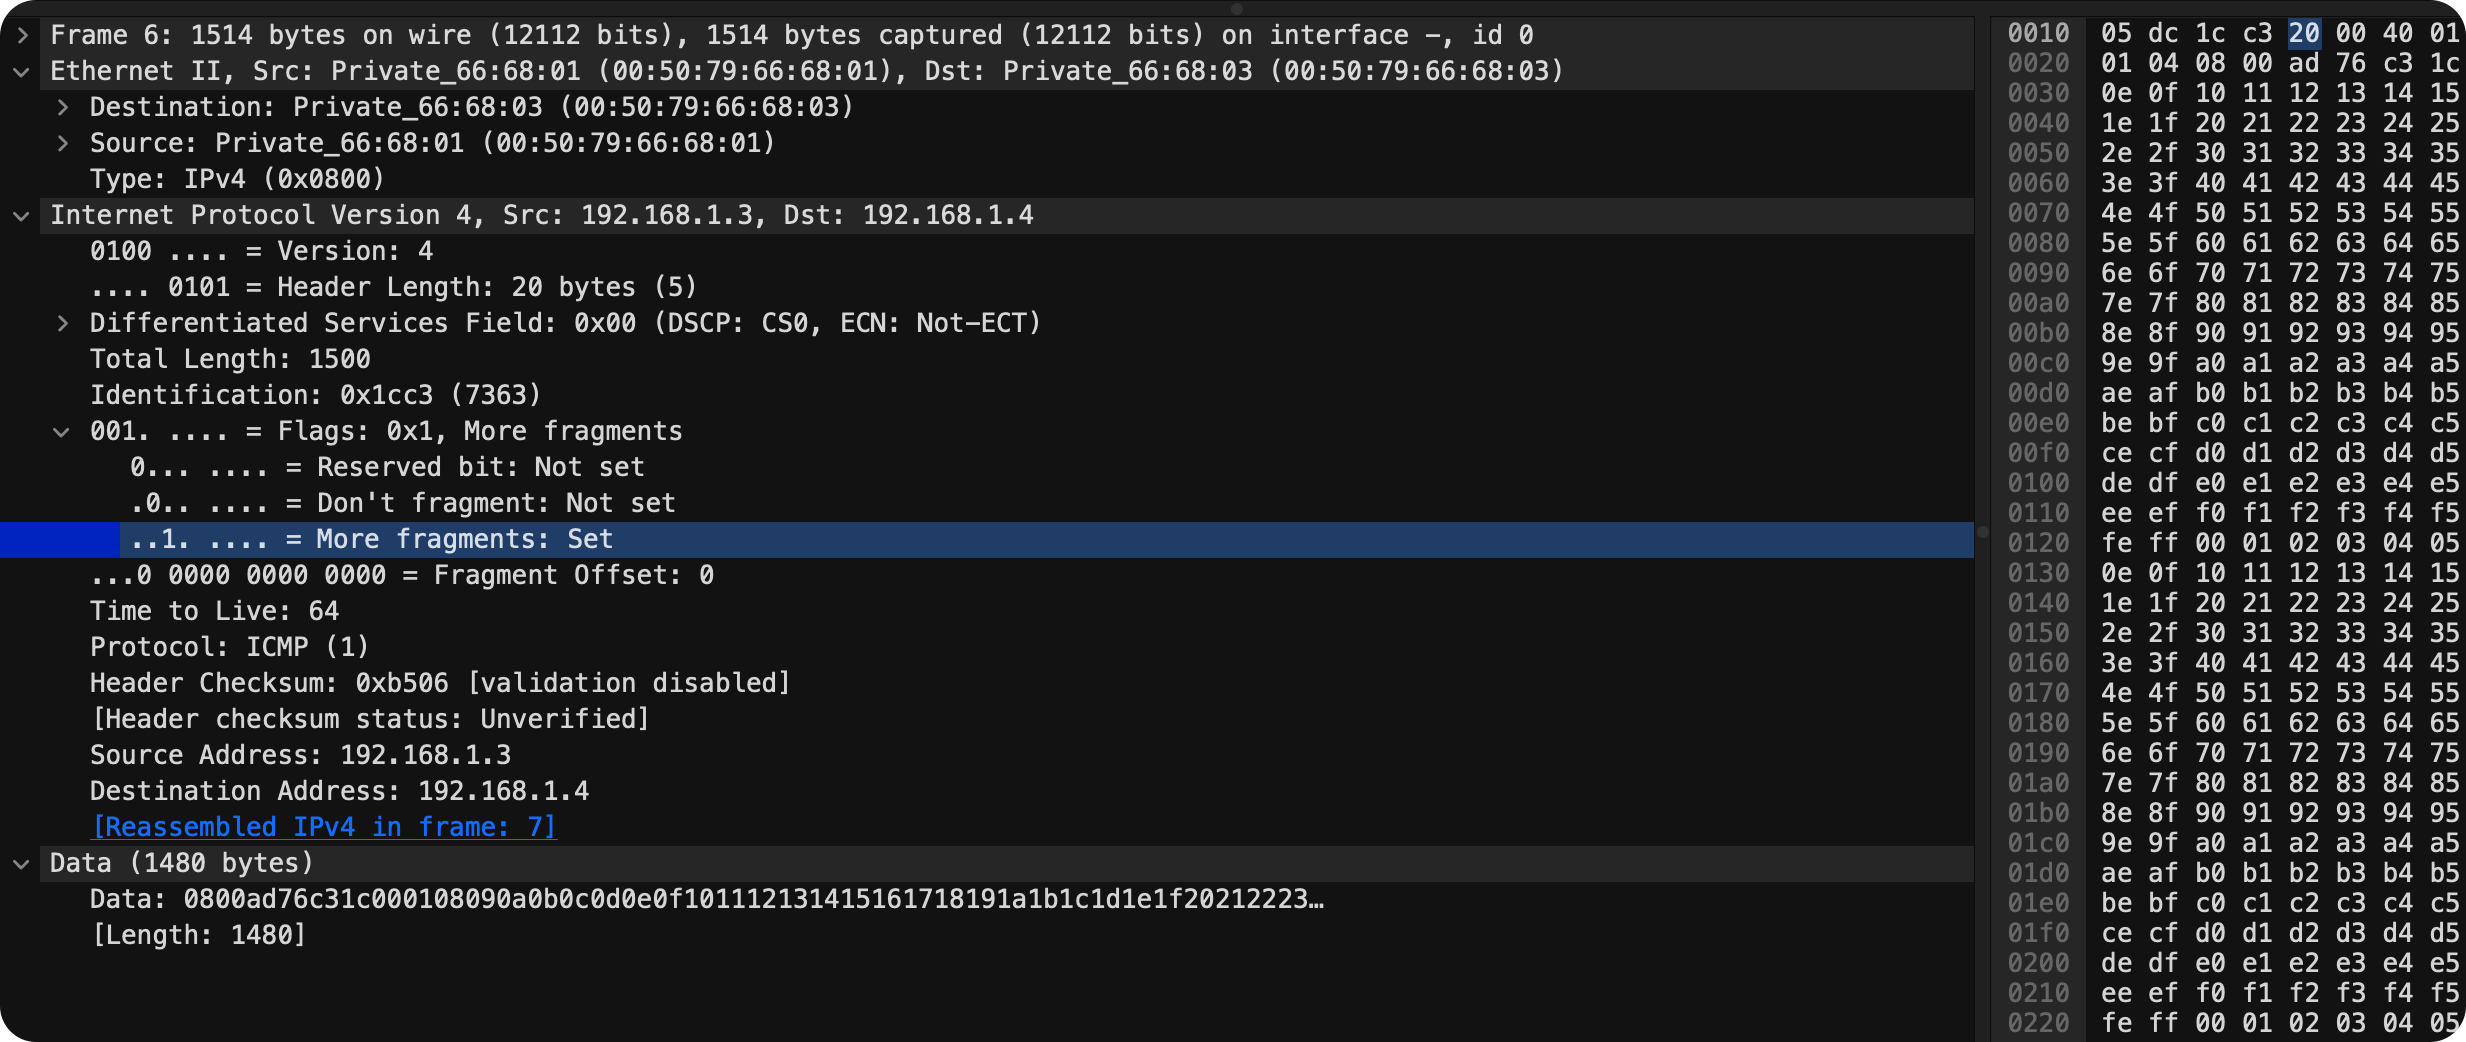
\includegraphics[width=10cm]{figure/2000_ipv4.png}
\caption{length=2000 第一个ipv4包}
\label{pic:2000_ipv4}
\end{figure}

在图\ref{pic:2000_icmp}中,MF位为0,DF位为0,说明该IP数据报是最后一个分片。其在ipv4层的标识也为0x1cc3(7363),偏移量为1480,说明该IP数据报是分片的。

可以看到有“IPv4 fragments”项目,其中写明了\#6(1480)和\#7(528)两个分片,其中\#6(1480)是第一个分片,\#7(528)是第二个分片。

且在该icmp数据帧,wireshark进行了frame 6 与frame 7的重组,重组后的ip数据报长度为2008字节,其结构为8个字节的icmp首部+2000个字节的icmp负载。



\begin{figure}[htb!]
  \centering
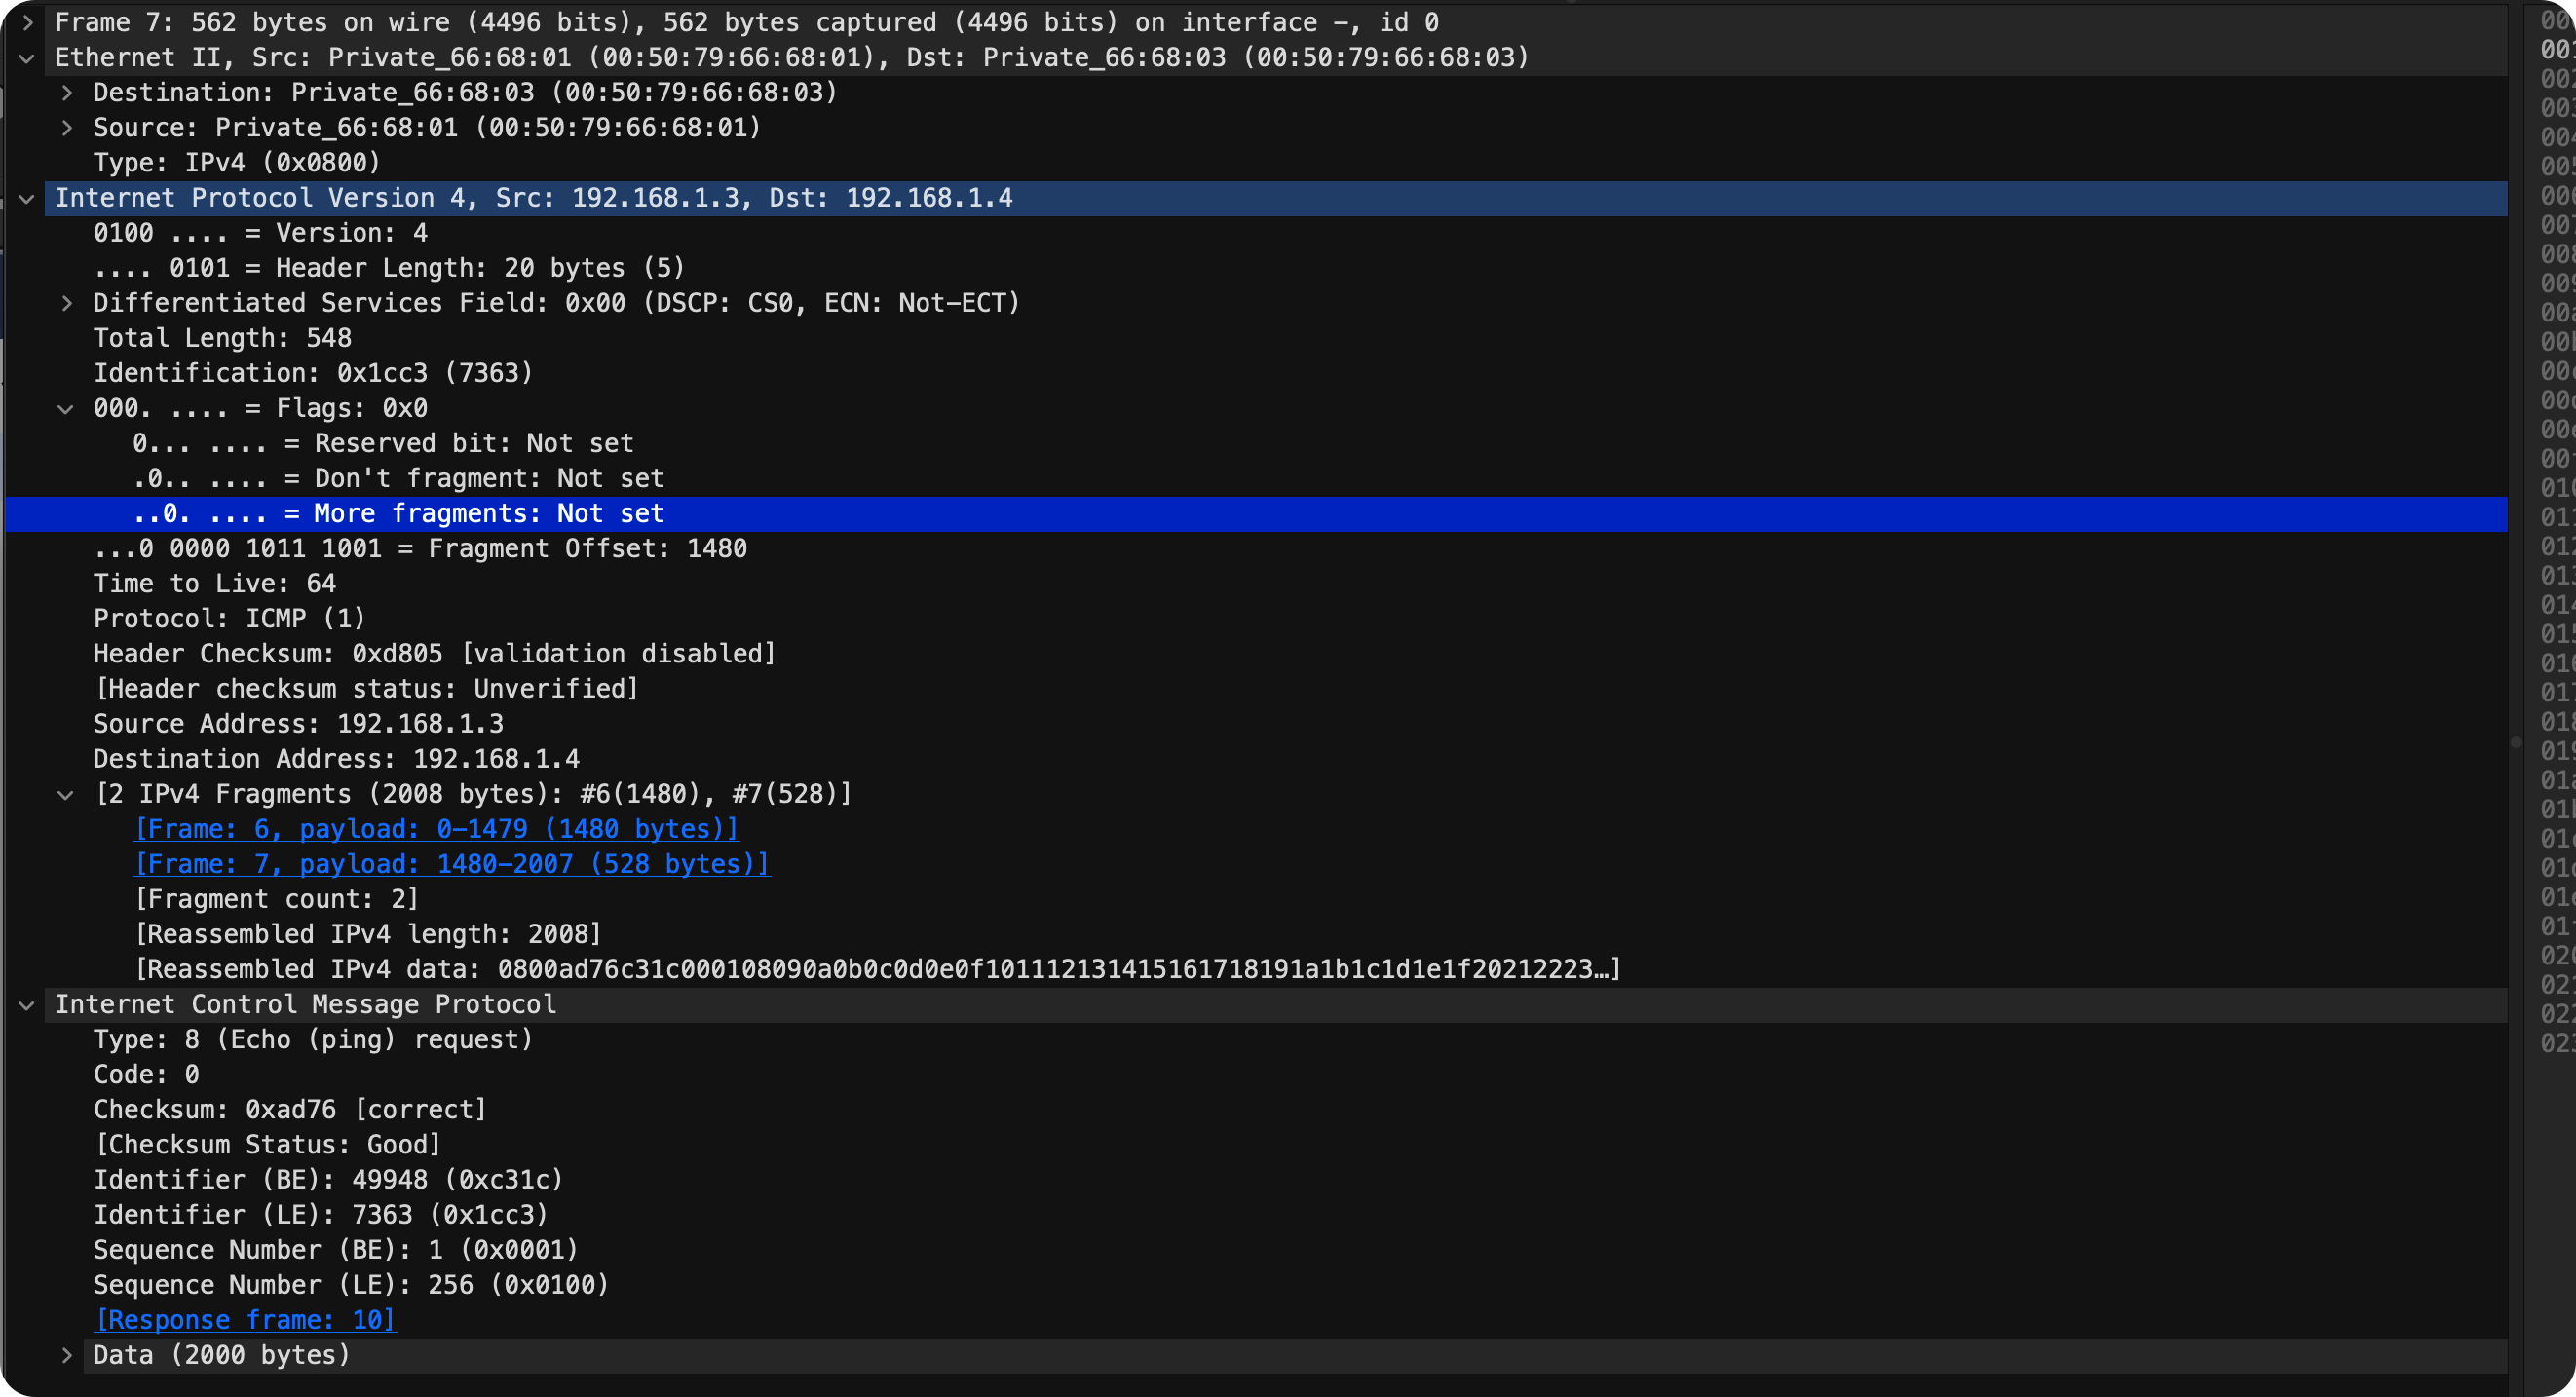
\includegraphics[width=10cm]{figure/2000_icmp.png}
\caption{length=2000 第2个icmp包}
\label{pic:2000_icmp}
\end{figure}


IPCM负载为2000时,可以看到ICMP报文发生分片,其中有一个IPv4数据帧,长度为1514字节,还有一个ICMP数据帧,长度为562字节,其结构为

icmp数据包分片出现ipv4数据帧的原因是:本身是一个ICMP协议数据报,现分成n片,切出后第1个分片会有ICMP报头,被识别ICMP协议;第2/3/4....n个分片没有ICMP报头,被识别为IP Fragment。

但是,在wireshark抓到的数据包中,第一个却被标识为ipv4,那么到底icmp报文在第几个分片中呢?我们分析负载数据部分来分析这个问题。

\begin{figure}[htb!]
  \centering
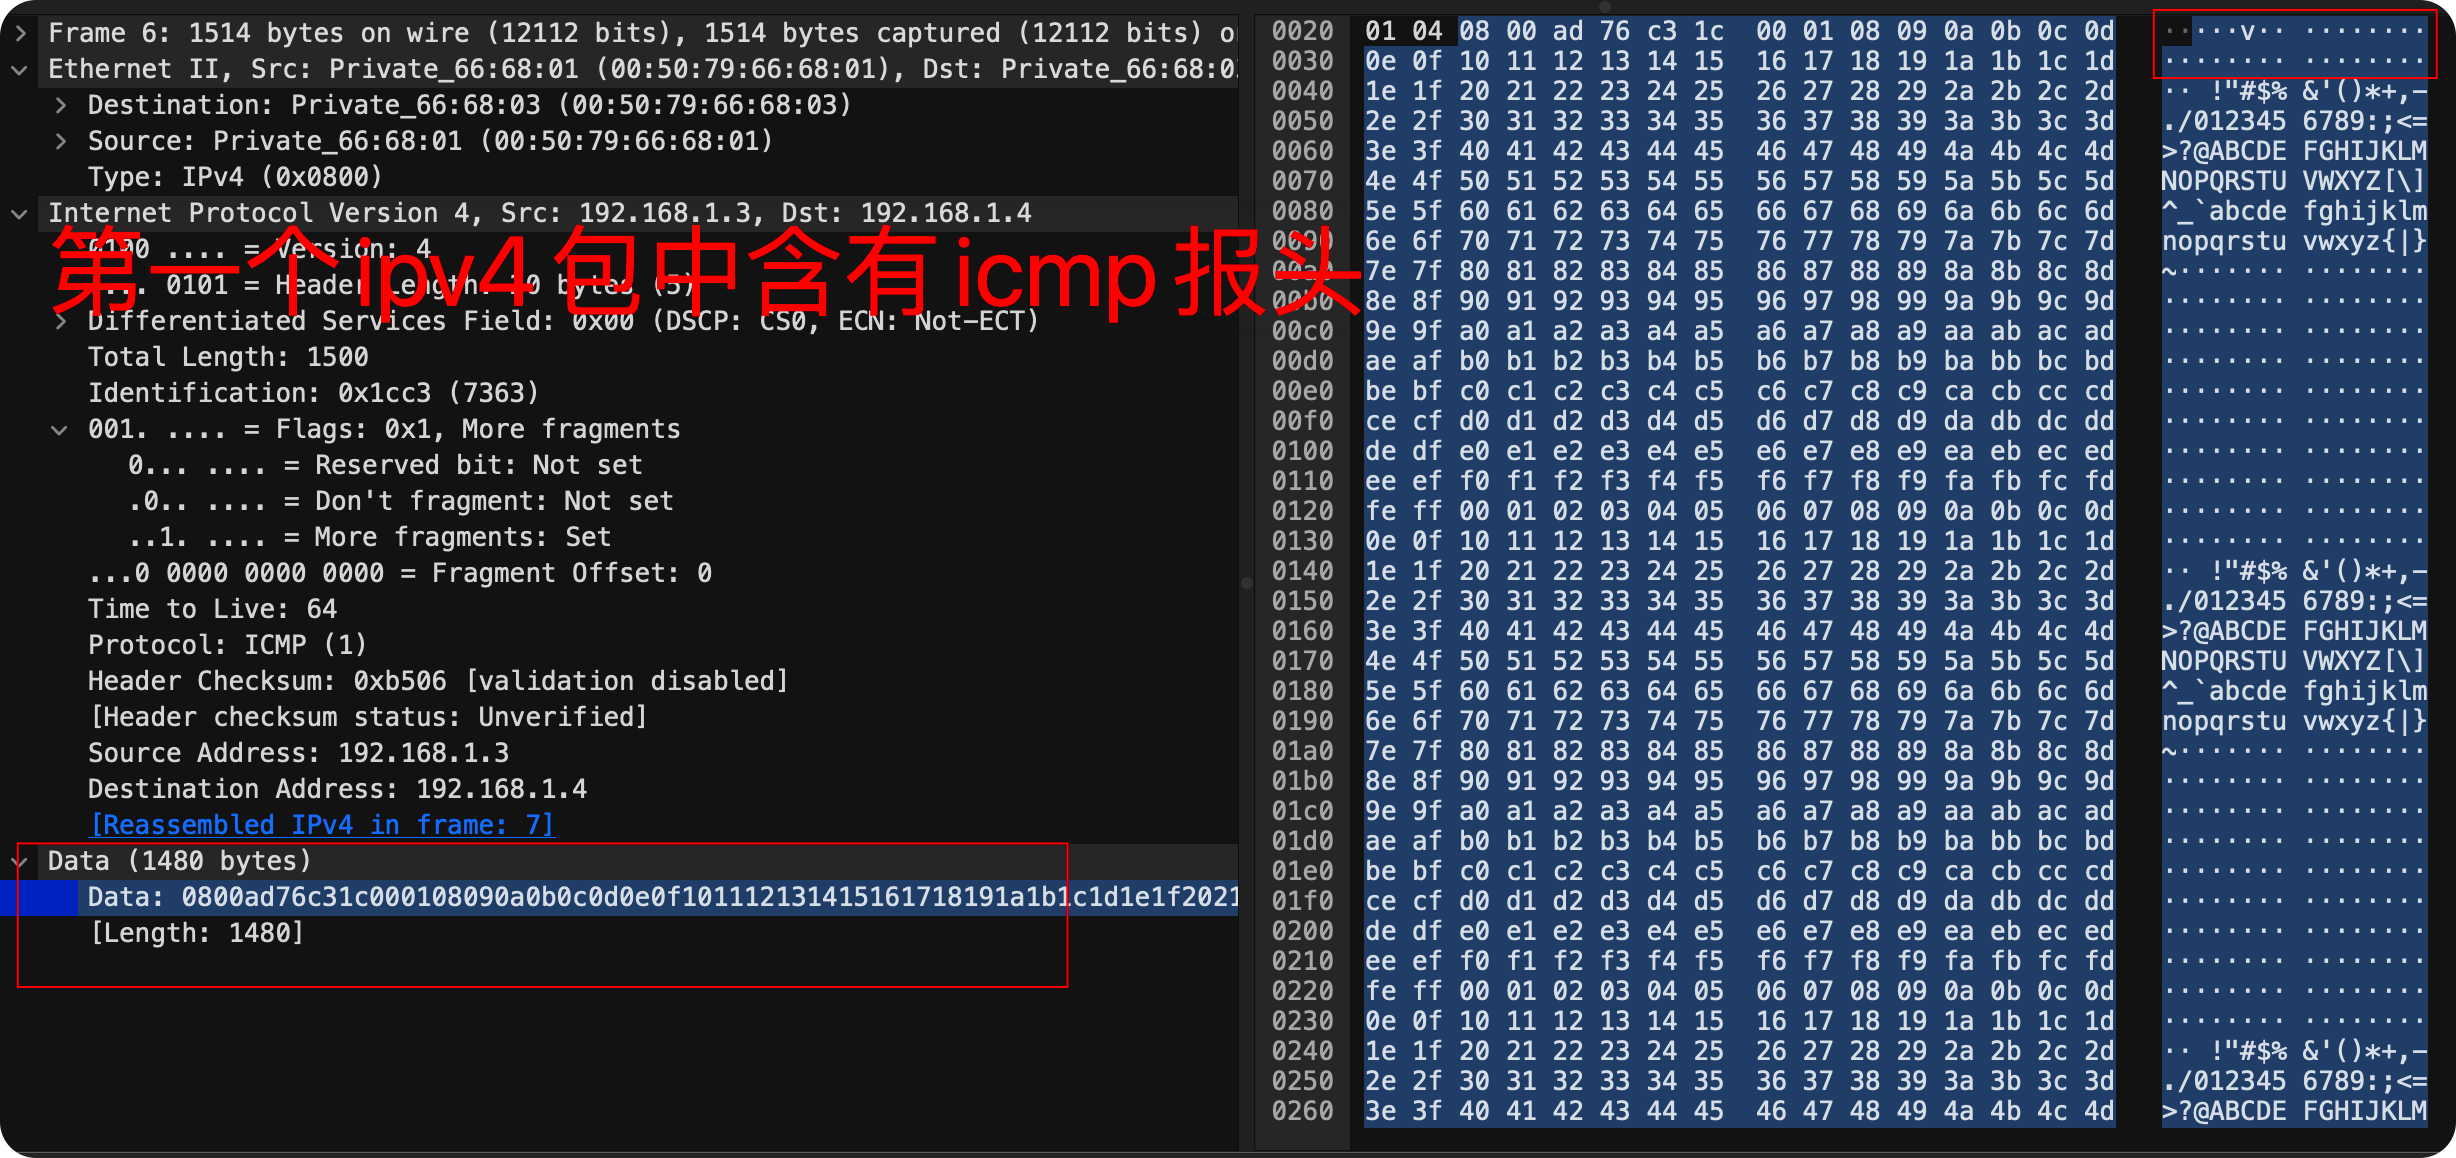
\includegraphics[width=10cm]{figure/2000_anly2.png}
\caption{第一个ipv4包data部分}
\label{pic:2000_ipv4_data}
\end{figure}

\begin{figure}[htb!]
  \centering
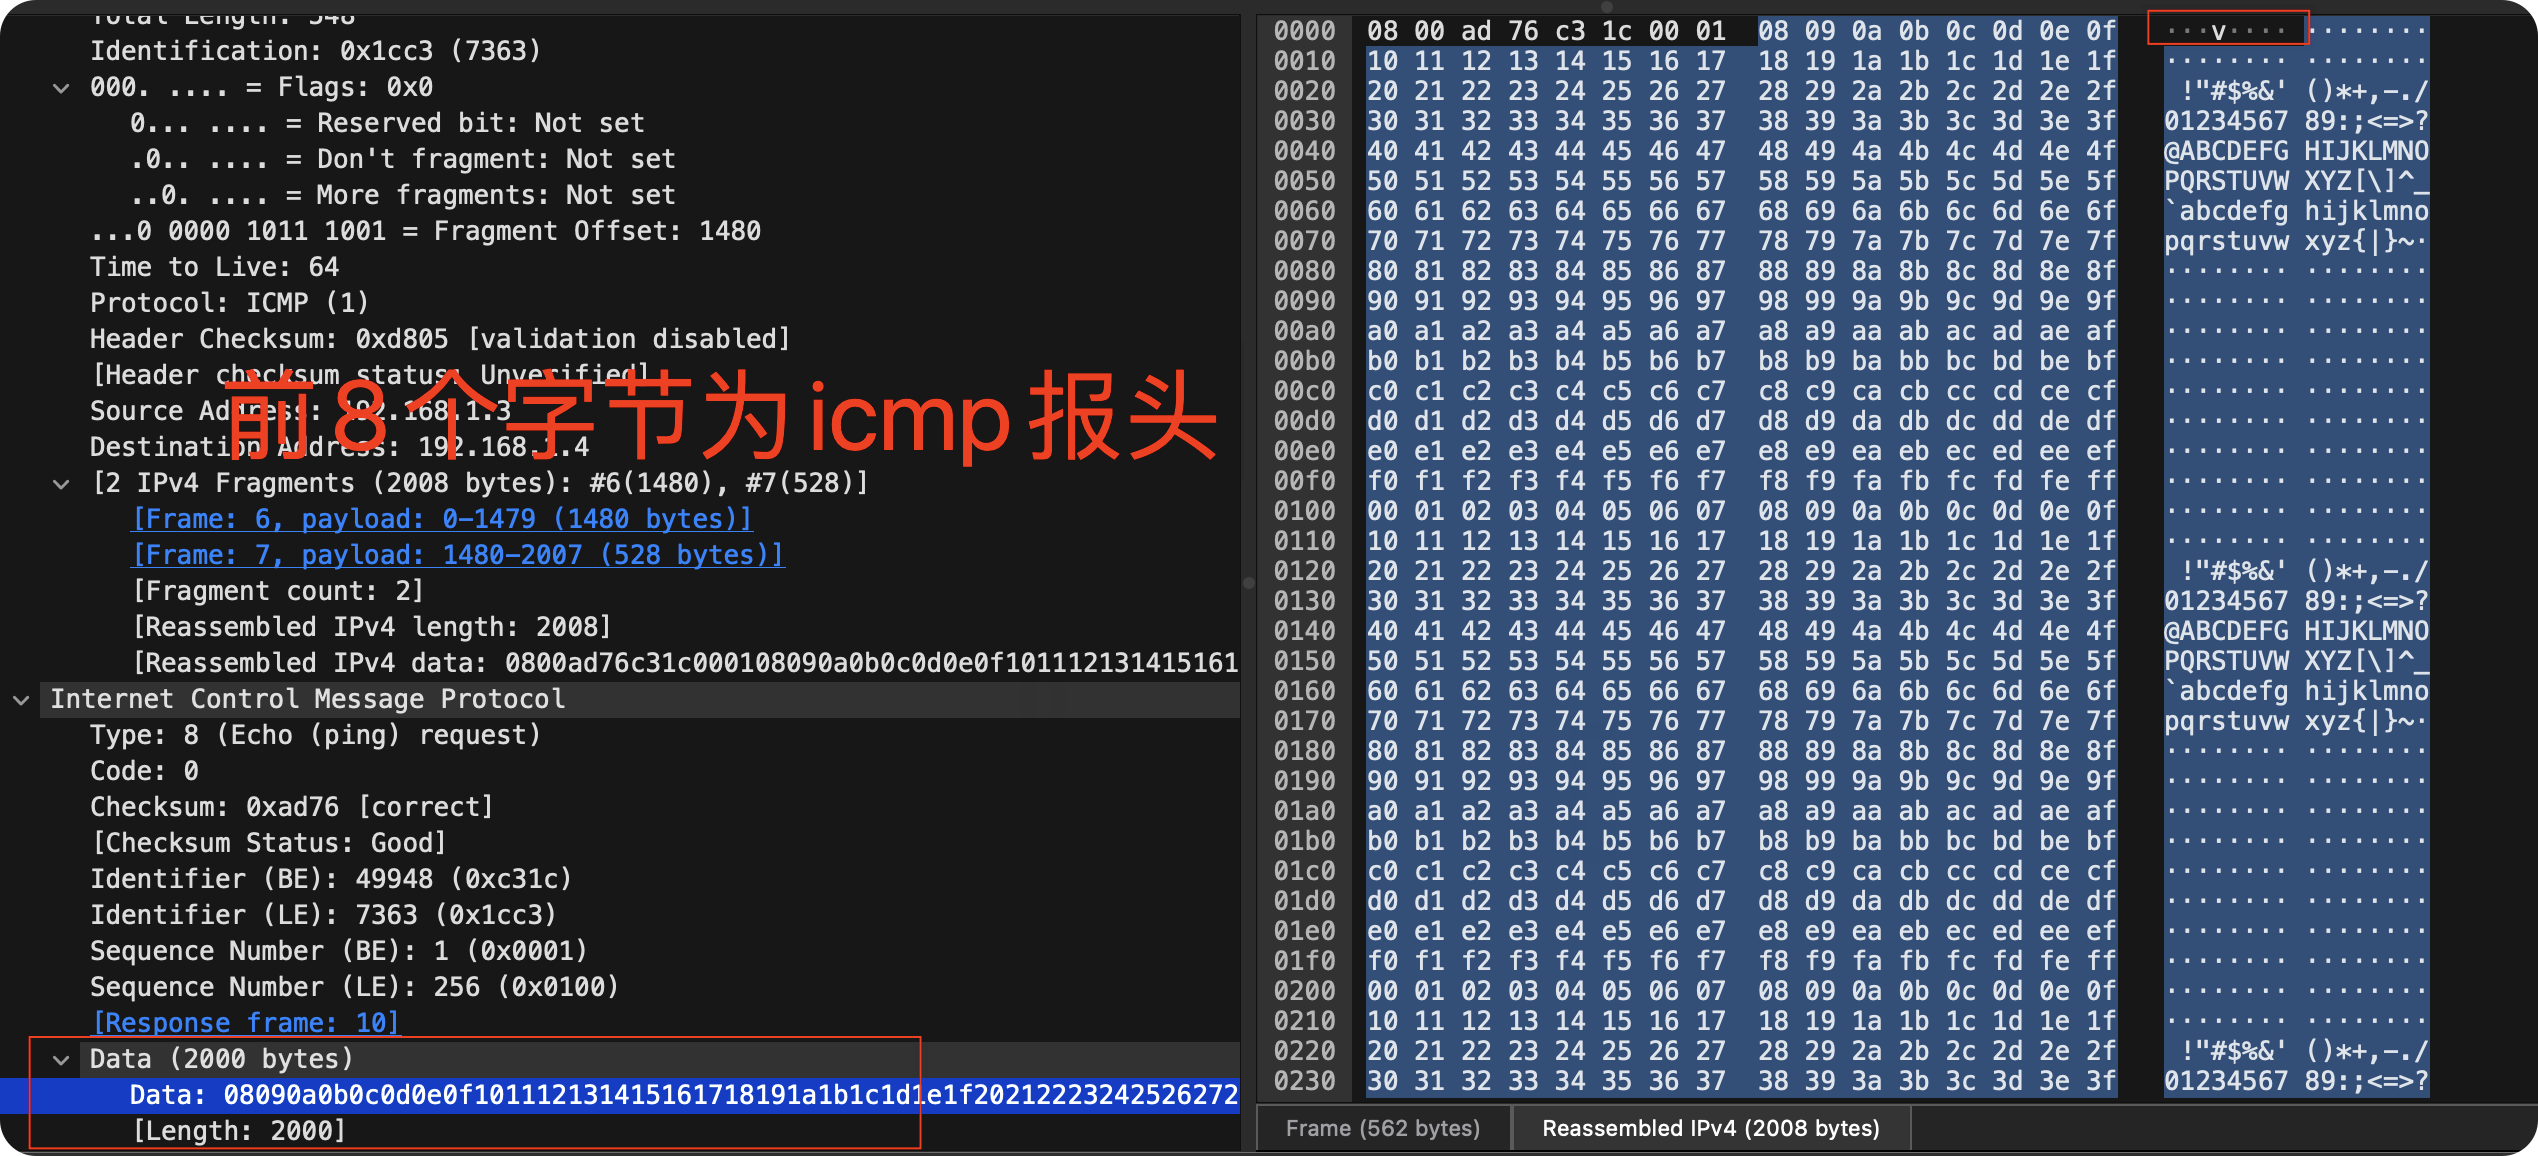
\includegraphics[width=10cm]{figure/2000_anly.png}
\caption{第二个icmp包data部分}
\label{pic:2000_icmp_data}
\end{figure}

如图\ref{pic:2000_ipv4_data}所示,第一个ipv4包的1480字节的data部分的前8个字 c3:1c:00:01 与图\ref{pic:2000_icmp_data}中完整的2000个字节的data数据的前八个字节并不一样,而与该data数据前面8个并不属于data数据的前八个字节 c3:1c:00:01 一样, 说明在第一个ipv4包中的前八个字节数据为icmp报头,后面的1472个字节为icmp报文负载部分。

但由于wireshark自动分析的结果,它自动属于某一个icmp数据包的分片data在最后一个分片重组展现出来,因此它将最后一个数据包标注为icmp数据帧,而将前面的所有分片(即使含有icmp报头)识别为ipv4,所以我们在最后一个帧字节长度仅有562的报文中,看到的是一个经过wireshark分析后的完整的icmp报文。

而事实上,icmp的报头在第一个ipv4包中,而第二个被识别为icmp的包中并没有icmp报头。则帧结构为:

第一个ipv4帧长度1514字节 = 以太网帧首部(14字节) + IP首部(20字节)+ ICMP首部(8字节)+ ICMP 负载长度(1472字节)

第2个icmp帧长度562字节 = 以太网帧首部(14字节) + IP首部(20字节) + ICMP负载长度(528字节)

分片前 ICMP报文负载数据长度为2000字节 = 1472字节 + 528 字节

\paragraph{IPCM负载为4000} 

如图\ref{pic:4000}所示,IPCM负载为4000时,可以看到ICMP报文发生分片,其中前两个是ipv4数据帧,长度为1514字节,还有一个ICMP数据帧,长度为1082字节。按照wireshark的分析规则,我们可以知道,icmp报头在第一个ipv4文件中,而在最后一个分片,所有分片将经过重组后展现出来,而最后一个数据包将被识别为icmp数据帧。

\begin{figure}[htb!]
  \centering
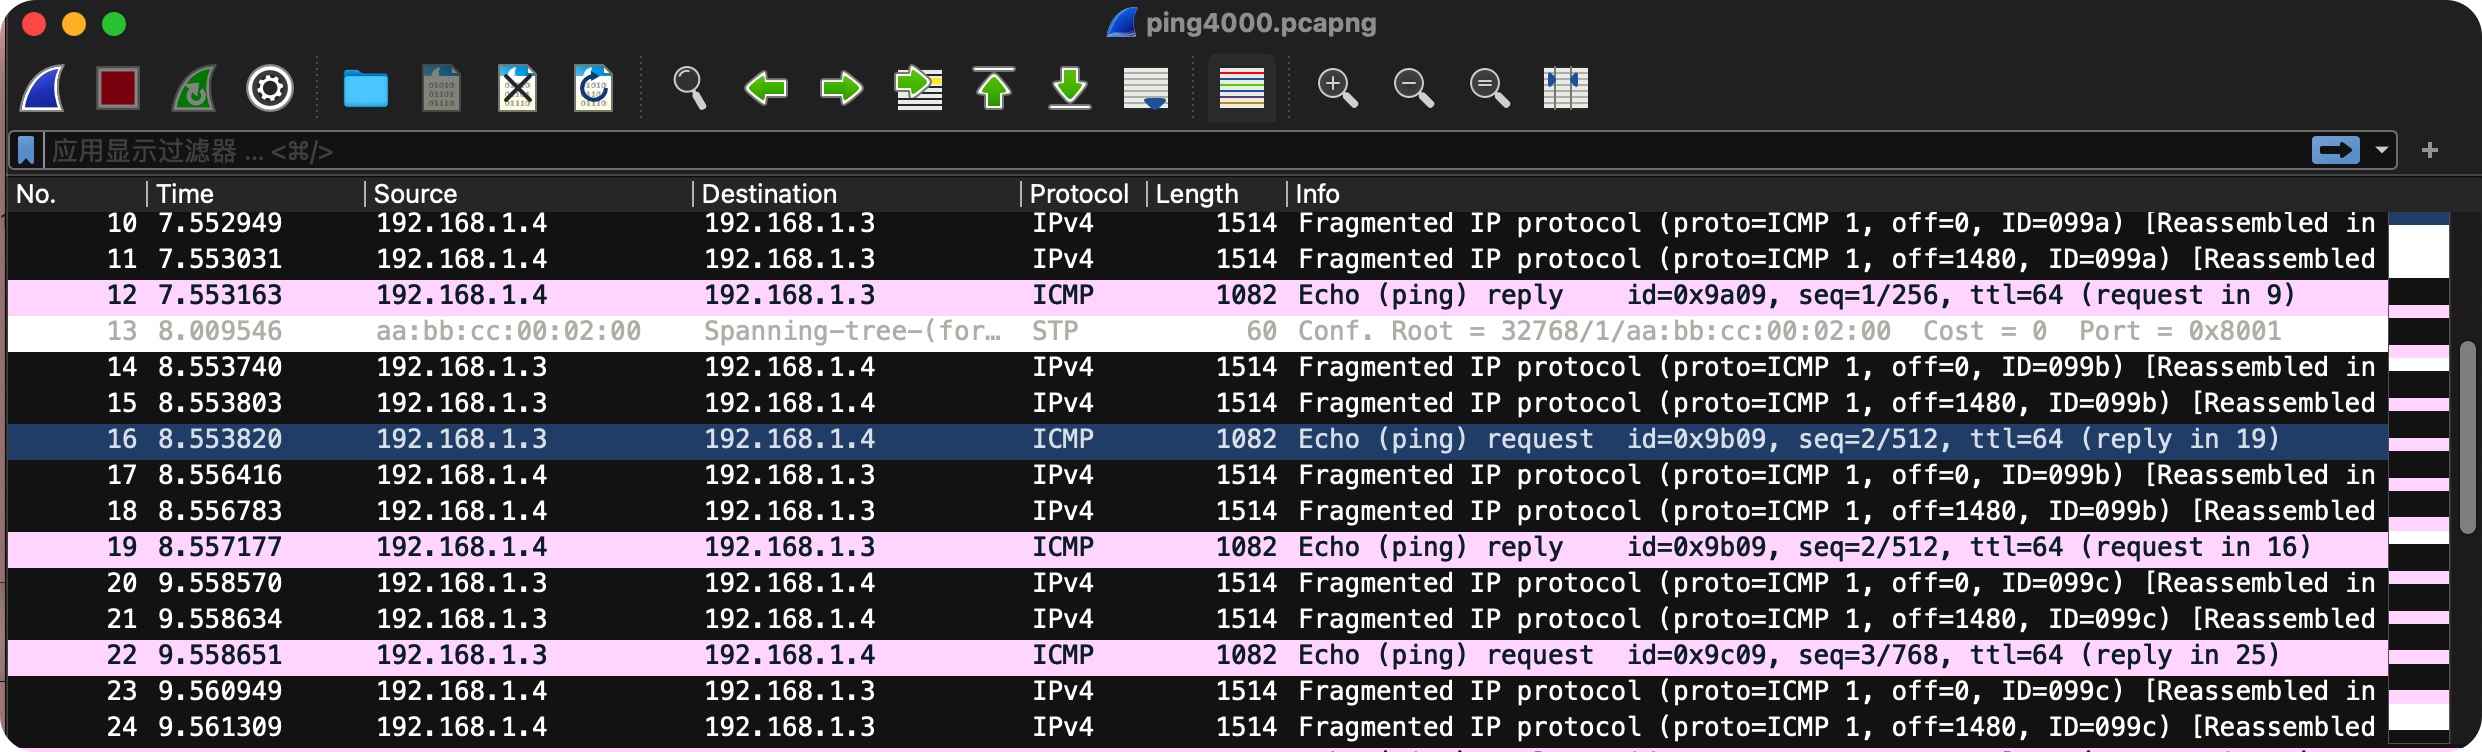
\includegraphics[width=10cm]{figure/ping4000.png}
\caption{length=4000}
\label{pic:4000}
\end{figure}

在图\ref{pic:4000-ipv4-01}中,indentfication:0x099a(2458),DF位为0,MF位为1,片偏移为0,说明该数据包为第一个分片,且该分片为不是最后一个分片。

当然,wireshark提供了蓝字分析标识了该frame 7 将在 frame 9 重组

ipv4帧长度1514字节 = 以太网帧首部(14字节) + IP首部(20字节)+ ICMP首部(8字节)+ ICMP 负载长度(1472字节)

其中的IP数据内容DATA长度(1480字节)=ICMP首部(8字节)+ ICMP 负载长度(1472字节)

\begin{figure}[htb!]
  \centering
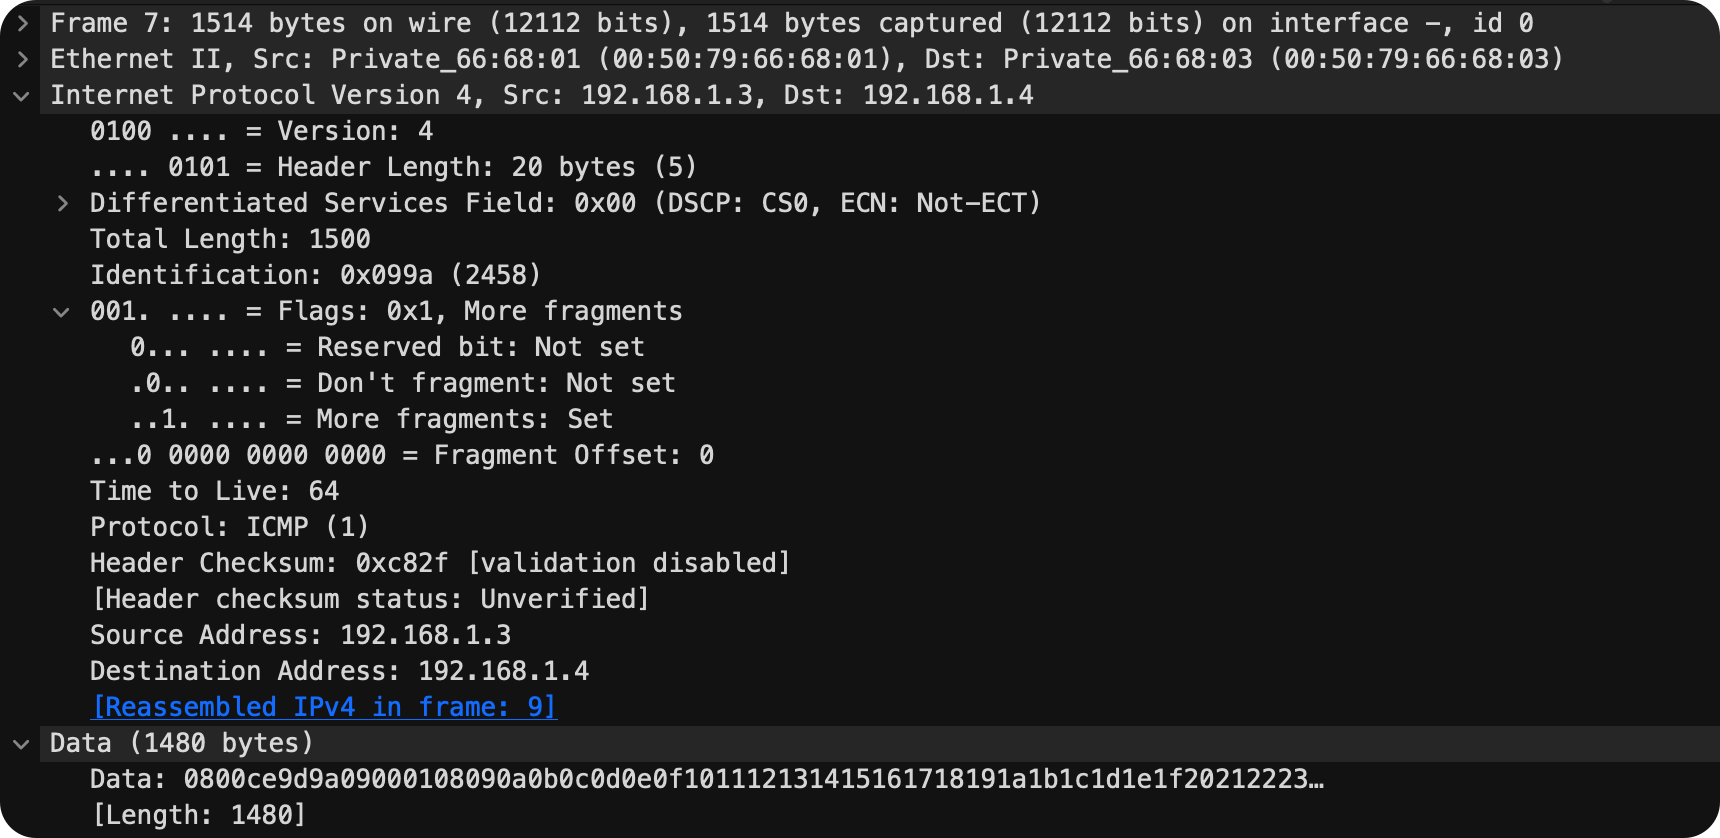
\includegraphics[width=10cm]{figure/4000_ipv4_01.png}
\caption{ping 4000-ipv4-01}
\label{pic:4000-ipv4-01}
\end{figure}

在图\ref{pic:4000-ipv4-02}中,indentfication:0x099a(2458),DF位为0,MF位为1,片偏移为1480,说明该数据包为第二个分片,且该分片为不是最后一个分片。

当然,wireshark提供了蓝字分析标识了该frame 8 将在 frame 9 重组

ipv4帧长度1514字节 = 以太网帧首部(14字节) + IP首部(20字节)+ ICMP 负载长度(1480字节)

其中的IP数据长度内容DATA长度(1480字节)= ICMP 负载长度(1480字节)



\begin{figure}[htb!]
  \centering
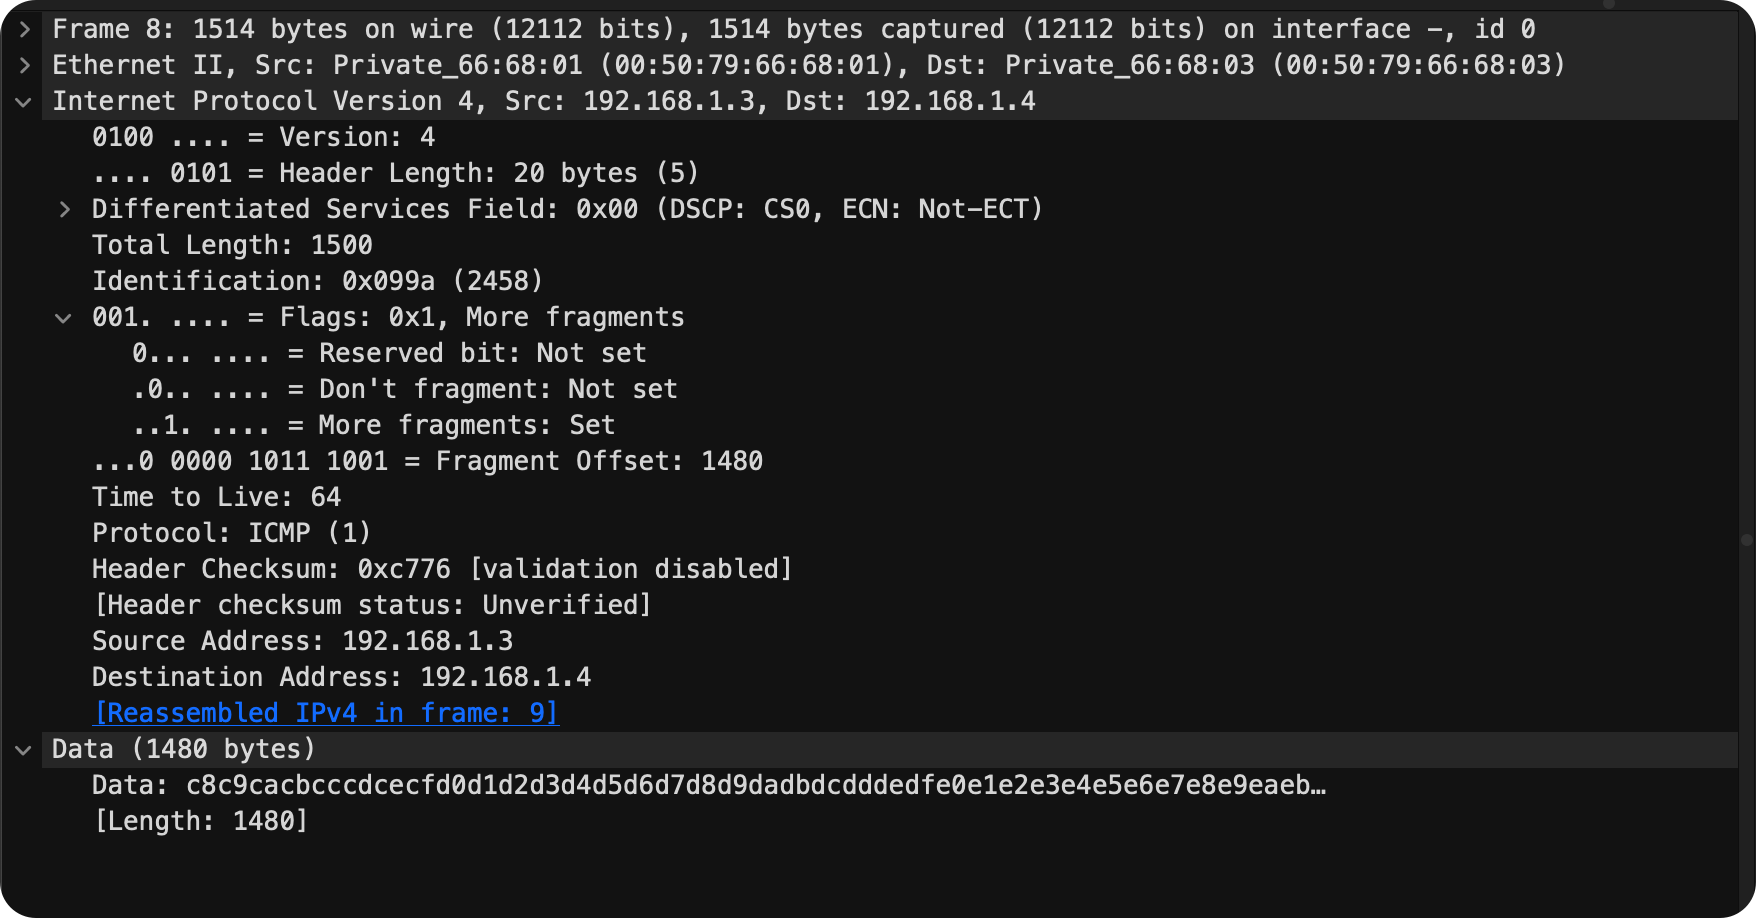
\includegraphics[width=10cm]{figure/4000_ipv4_02.png}
\caption{ping 4000-ipv4-02}
\label{pic:4000-ipv4-02}
\end{figure}

在图\ref{pic:4000-icmp}中,indentfication:0x099a(2458),DF位为0,MF位为0,片偏移为2960,说明该数据包为最后一个分片。

当然,wireshark提供了蓝字分析了有3个IPv4 Fragments(4008 bytes):\#7(1480),\#8(1480),\#9(1048)。

将IPv4 data重组后得到4008个字节=8字节ICMP首部+4000字节ICMP负载。

该icmp帧长度1082字节 = 以太网帧首部(14字节) + IP首部(20字节)+ ICMP 负载长度(1048字节)

该帧的IP数据内容DATA长度(1048字节)= ICMP 负载长度(1048字节)
\begin{figure}[htb!]
  \centering
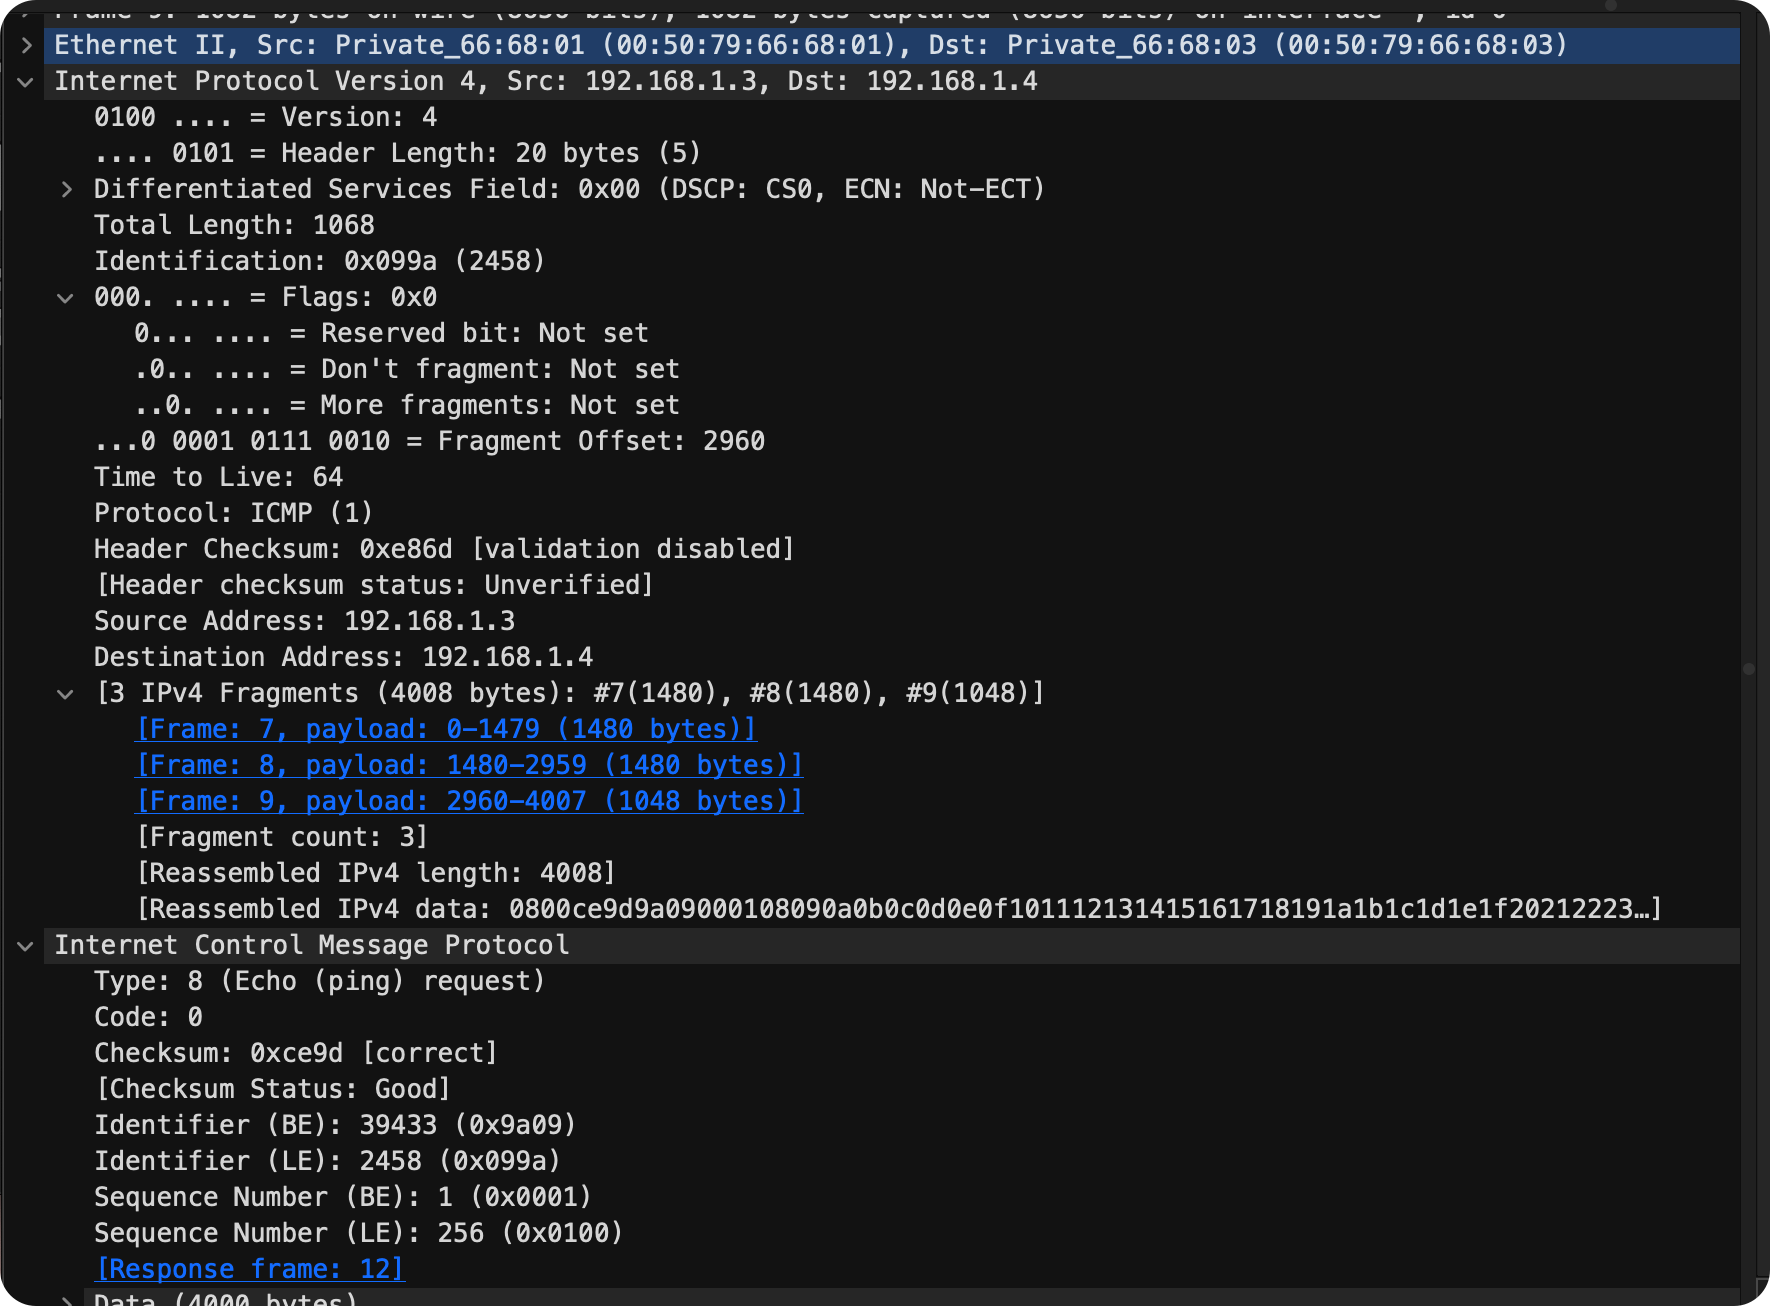
\includegraphics[width=10cm]{figure/4000_icmp.png}
\caption{ping 4000-icmp}
\label{pic:4000-icmp}
\end{figure}




\subsection{执行 Tracert 命令,观察 ICMP 差错报文的结构,并分析其工作原理}

\subsubsection{ICMP 差错报文原理}

\begin{figure}[htb!]
  \centering
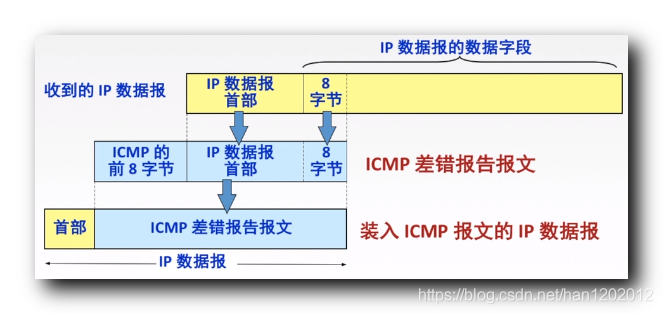
\includegraphics[width=10cm]{figure/icmp-struct.png}
\caption{ICMP 差错报文形成}
\label{pic:icmp-struct}
\end{figure}
\paragraph*{ICMP 差错报文形成 }

如图\ref{pic:icmp-struct},是ICMP差错报文形成的过程。

1. 取出 IP 数据报内容 : 取出 IP 数据报首部 , 以及 数据部分的前 8 字节 ;

2. ICMP 差错报文组成 : ICMP 前 8 个字节 + IP 数据报首部 + IP 数据报数据部分前 8 字节 ;

3. 组装 IP 数据报 : 将 ICMP 数据报装入 IP 数据报数据部分 ;

\paragraph*{[ICMP time exceeded] 超时类ICMP差错报文}

ICMP差错报告报文主要在以下几种情况中,会发送ICMP超时报文: 

1. 当路由器接收到的数据报的TTL生命周期字段值为0时,路由器会把该数据报丢弃掉,并向源主机发回一个ICMP超时报文。

2. 当目标主机在规定时间内没有收到所有的数据分片时,会把已经收到的所有数据分片丢弃,并向源主机发回一个ICMP超时报文。在超时报文中,代码0只能给路由器使用,表示生存周期字段值为0,代码1只能给目的主机使用,它表示在规定的时间内,目的主机没有收到所有的数据分片。 
\begin{figure}[htb!]
  \centering
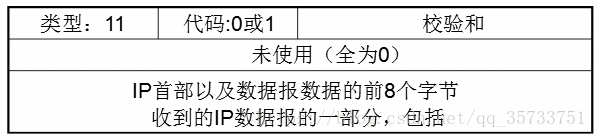
\includegraphics[width=10cm]{figure/outoftime.png}
\caption{超时报文}
\label{pic:time}
\end{figure}
 

ICMP超时报文的类型值是11,code的值有可能是0或者是1,其中标识符和序列号全部填充为0。


\paragraph*{[ICMP unreachable] 不可达类ICMP差错报文}
不可达类ICMP差错报文的Type值是3,Code值有可能是0、1、2、3、4等。

\subparagraph{[ICMP Network unreachable] 网络不可达类ICMP差错报文}
Code值为0,表示网络不可达。
IP 地址是分为网络号和主机号的,所以当路由器中的路由器表匹配不到接收方 IP 的网络号,就通过 ICMP 协议以网络不可达(Network Unreachable)的原因告知主机。
自从不再有网络分类以后,网络不可达也渐渐不再使用了。


\subparagraph{[ICMP Host unreachable] 主机不可达类ICMP差错报文}

Code值为1,表示主机不可达。
当路由表中没有该主机的信息,或者该主机没有连接到网络,那么会通过 ICMP 协议以主机不可达(Host Unreachable)的原因告知主机。
\subparagraph{[ICMP Protocol unreachable] 协议不可达类ICMP差错报文}
Code值为2,表示协议不可达。
当主机使用 TCP 协议访问对端主机时,能找到对端的主机了,可是对端主机的防火墙已经禁止 TCP 协议访问,那么会通过 ICMP 协议以协议不可达的原因告知主机。

\subparagraph{[ICMP Port unreachable] 端口不可达类ICMP差错报文}
Code值为3,表示端口不可达。
ICMP数据包 "Destination Port Unreachable "告诉我们,从我们的计算机发出的ping请求无法进入目标主机上对应的端口号。这意味着从你的计算机发送的数据包成功地到达了目标主机,但它未能被目标端口号处理。这种情况下,目标主机会向源主机发送一个ICMP Destination Port Unreachable差错报文,告诉源主机,目标主机上对应的端口号无法处理该报文。

这种情况发生的可能原因是目标主机上没有对该端口号的监听。

也就是 当主机访问对端主机 8080 端口时,这次能找到对端主机了,防火墙也没有限制,可是发现对端主机没有进程监听 8080 端口,那么会通过 ICMP 协议以端口不可达的原因告知主机。



\subsubsection{路由追踪程序traceroute/tracert}

Traceroute是Linux和Mac OS等系统默认提供的路由追踪小程序,Tracert是Windows系统默认提供的路由追踪小程序。二者的功能相同,都能探测数据包从源地址到目的地址经过的路由器的IP地址。Traceroute/Tracert的实现都借助了TTL:通过向目的地址发送一系列的探测包,设置探测包的TTL初始值分别为1,2,3…,根据返回的超时通知(ICMP Time Exceeded Message)得到源地址与目的地址之间的每一跳路由信息。虽然两者输出结果一致,但在实现原理上还有着显著的差别。

\paragraph*{Traceroute实现原理}

Linux和Mac OS等系统使用UDP包进行探测,目标端口号默认为33434,每次探测目标端口号加1。Traceroute故意使用了一个大于 30000 的目标端口号,以保证目标地址收到数据包后能够返回一个“端口不可达”的 ICMP 报文,于是源地址就可将端口不可达报文当作跟踪结束的标志。

Traceroute每跳默认发送3个探测包(发包的数量可通过-q进行设置),探测包的返回会受到网络情况的影响。如果防火墙封掉了ICMP的返回信息,那么相应的延时位置会以*显示。如果某台网关阻塞或者某台DNS出现问题,那么相应行的延时会变长。可以加-n 参数来避免DNS解析,以IP格式输出数据。

每个探测包都有唯一的标识号,使得Traceroute能够识别返回的包。UDP数据包使用递增的目标端口号进行标识。

\begin{figure}[htb!]
  \centering
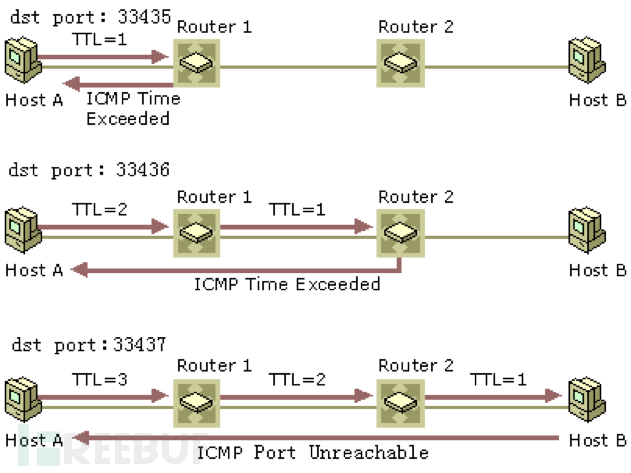
\includegraphics[width=10cm]{figure/traceroutes-why.jpeg}
\caption{Traceroute实现原理}
\label{pic:traceroute}
\end{figure}

如图\ref{pic:traceroute},是使用Traceroute实现路由信息的原理步骤:

1. 从源地址发出一个UDP探测包到目的地址,并将TTL设置为1;

2. 到达路由器时,将TTL减1;

3. 当TTL变为0时,包被丢弃,路由器向源地址发回一个ICMP超时通知(ICMP Time Exceeded Message),内含发送IP包的源地址,IP包的所有内容及路由器的IP地址;

4. 当源地址收到该ICMP包时,显示这一跳路由信息;

5. 重复1~5,并每次设置TTL加1;

6. 直至目标地址收到探测数据包,并返回端口不可达通知(ICMP Port Unreachable);

7. 当源地址收到ICMP Port Unreachable包时停止traceroute。

\paragraph*{Tracert实现原理}

Windows系统使用ICMP请求回显(ICMP Echo Request)数据包进行探测,源地址以目的地址返回的ICMP回应答复(ICMP Echo Reply)作为跟踪结束标志。

Tracert每跳默认发送3个探测包。在未能到达路由器或未返回ICMP超时通知的情况下,相应的延时位置会以*显示。

每个探测包都有唯一的标识号,ICMP数据包使用seq进行标识。

\begin{figure}[htb!]
  \centering
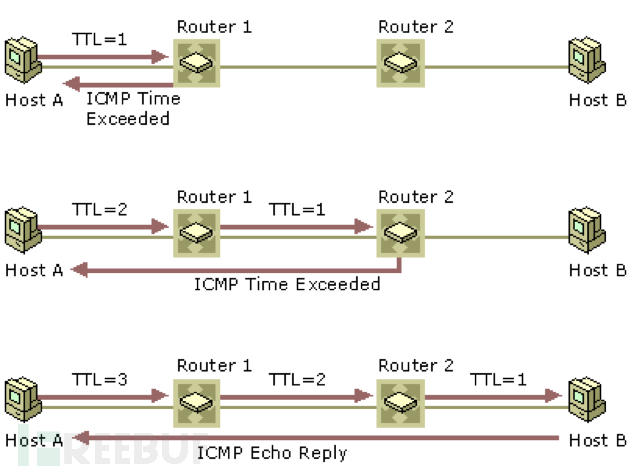
\includegraphics[width=10cm]{figure/tracert-why.jpeg}
\caption{Tracert实现原理}
\label{pic:tracert}
\end{figure}


如图\ref{pic:tracert},是使用Tracert实现路由信息的原理步骤:

1. 从源地址发出一个ICMP请求回显(ICMP Echo Request)数据包到目的地址,并将TTL设置为1;

2. 到达路由器时,将TTL减1;

3. 当TTL变为0时,包被丢弃,路由器向源地址发回一个ICMP超时通知(ICMP Time Exceeded Message),内含发送IP包的源地址,IP包的所有内容及路由器的IP地址;

4. 当源地址收到该ICMP包时,显示这一跳路由信息;

5. 重复1~5,并每次设置TTL加1;

6. 直至目标地址收到探测数据包,并返回ICMP回应答复(ICMPEcho Reply);

7. 当源地址收到ICMP Echo Reply包时停止tracert。

\paragraph*{Tracert出现请求超时的原因}

Tracert路由跟踪图上返回的延时是基于ICMP协议的,相当于去ping每一个节点IP;出现超时、延时大的原因有以下几点因素

1、超时的节点设备如网络设备路由器、服务器等做了安全设置,禁止ICMP协议,即禁ping;

2、超时的节点网络拥塞或者网络质量差延时过大所致;

3、超时的节点设备宕机、关机等对ICMP协议无法响应;

4、电信,联通等国际出口骨干延时太大。

基于UDP探测包的Traceroute也是同理。

\subsubsection{使用Windows 实现 Tracert www.baidu.com}

启动 Wireshark 软件,选择要监听的网络接口,设置过滤条件 icmp。

在终端中使用 tracert 命令,目的主机是外网的一台设备(如图\ref{pic:tracertbaidu},tracert www.baidu.com)。


\begin{figure}[htb!]
  \centering
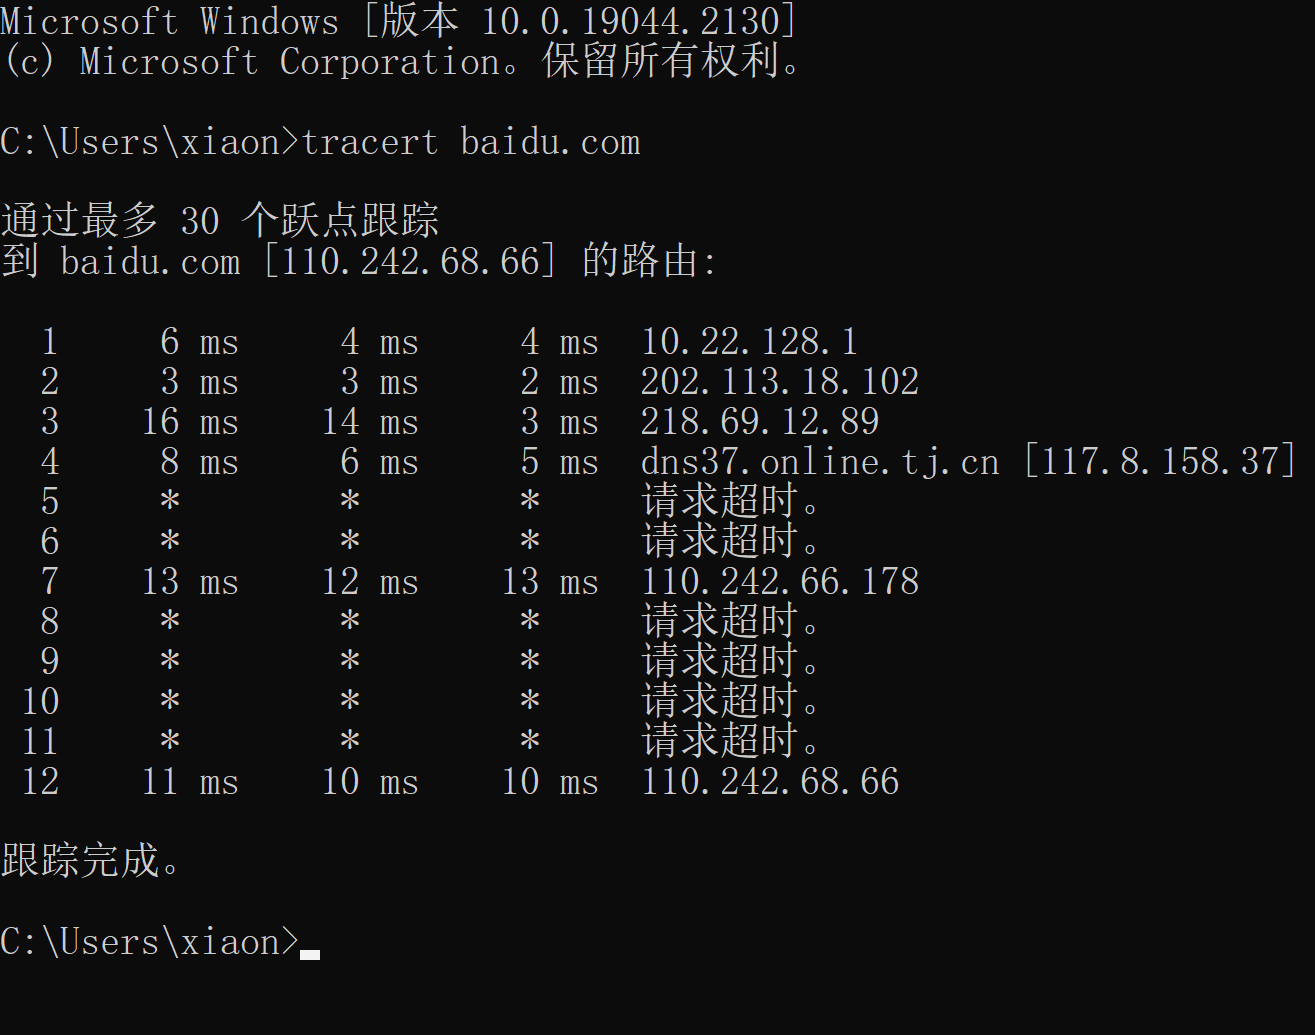
\includegraphics[width=10cm]{figure/tracertbaidu.png}
\caption{tracert baidu.com}
\label{pic:tracertbaidu}
\end{figure}



\subsubsection{分析ICMP 差错报文}

点击 Internet Control Message Protocol 展开,查看 ICMP 差错报文。得到的ICMP报文如图\ref{pic:tracertwrong}所示,其中有好几种类型的ICMP报文。

\begin{figure}[htb!]
  \centering
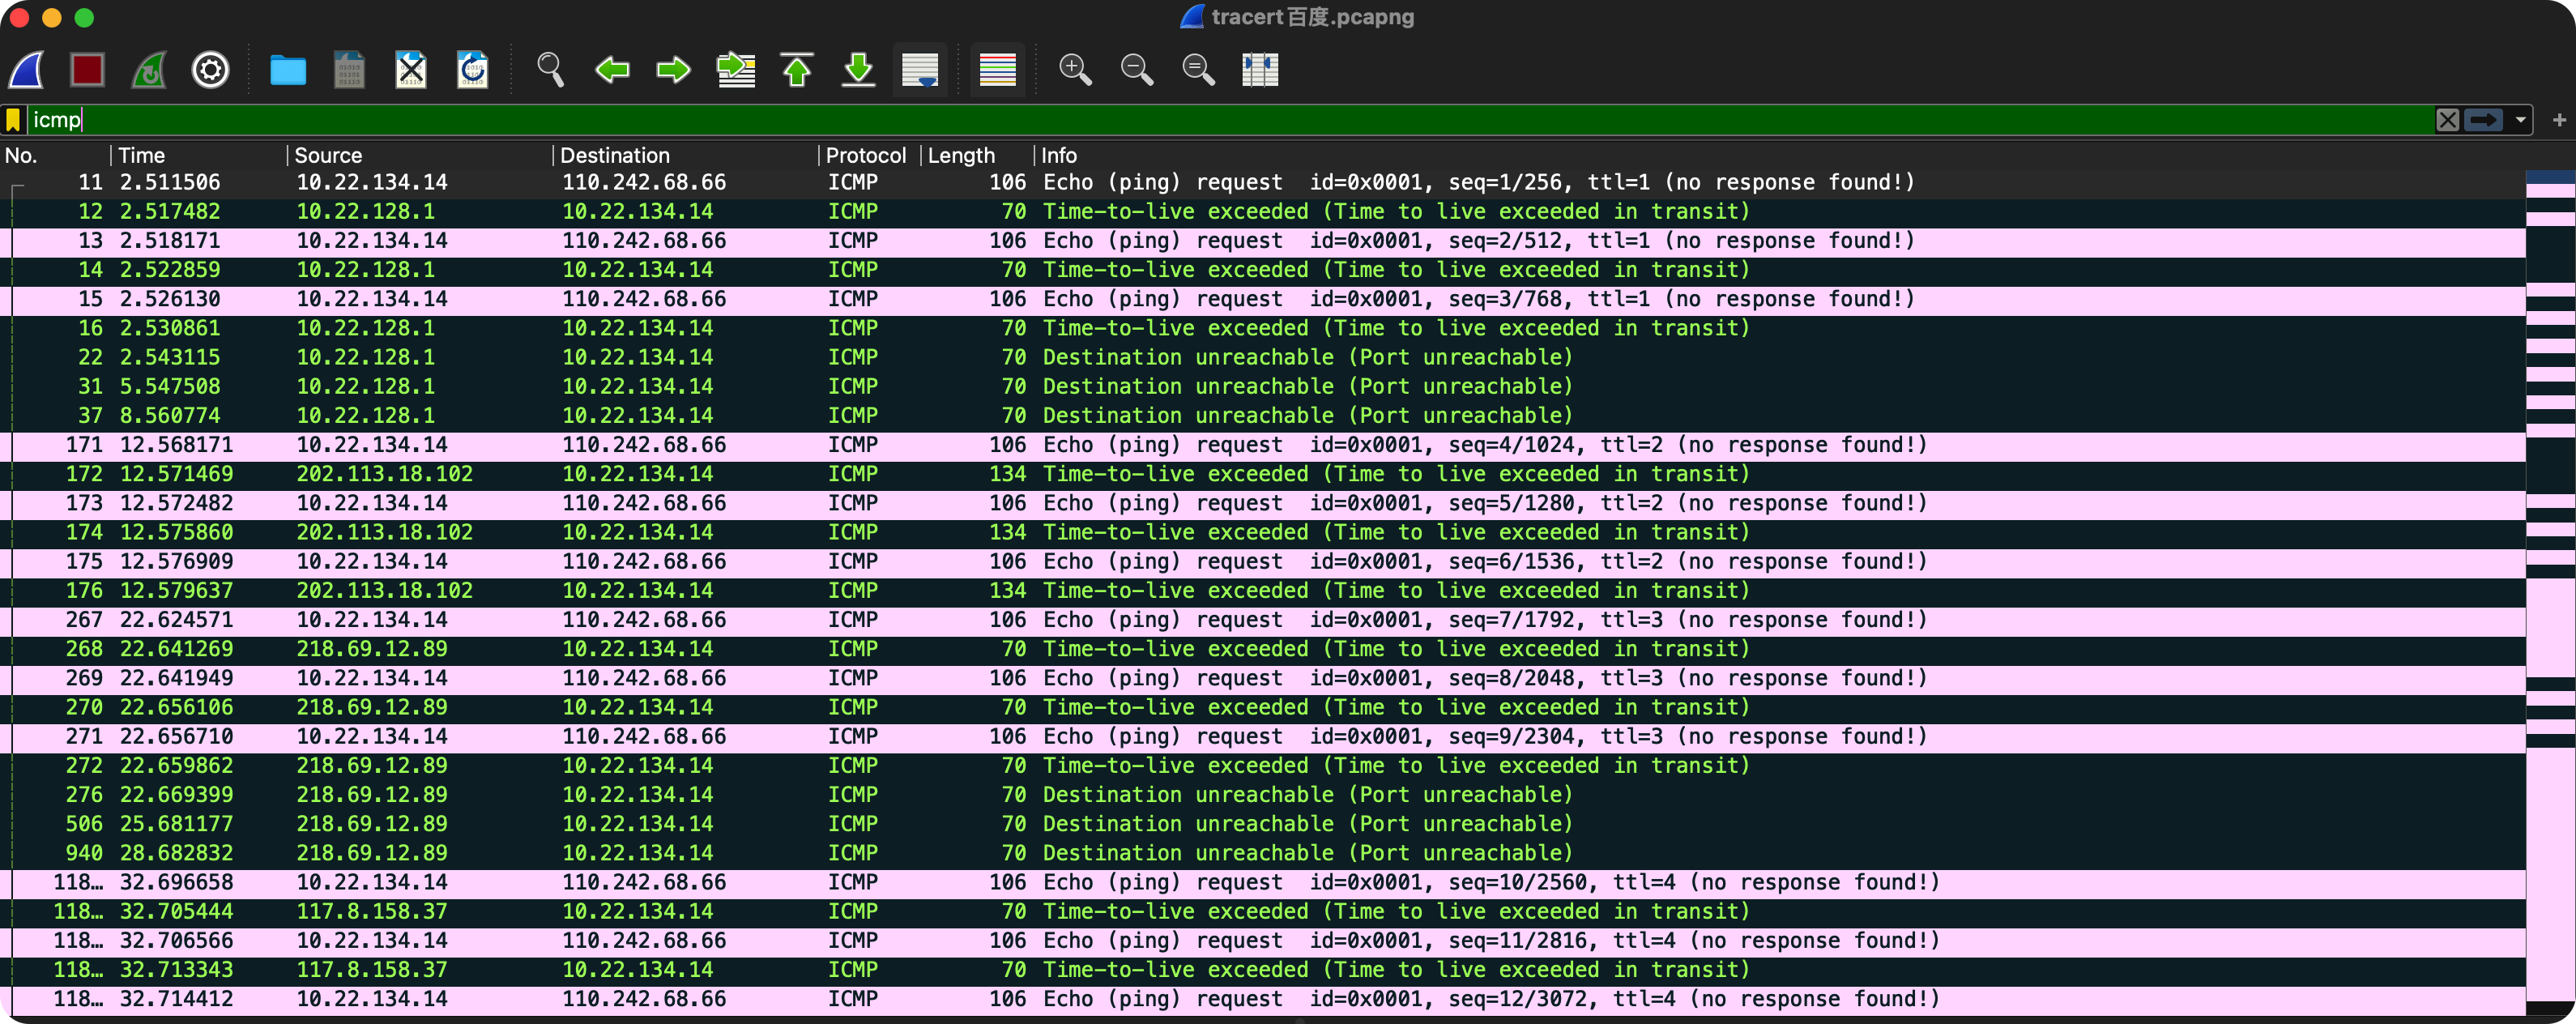
\includegraphics[width=10cm]{figure/tracert-wrong.png}
\caption{tracert baidu.com detail}
\label{pic:tracertwrong}
\end{figure}
观察并解释 ICMP 报文结构和字段内容:

\paragraph*{[ICMP time exceeded] 超时类ICMP差错报文}

\begin{figure}[htb!]
  \centering
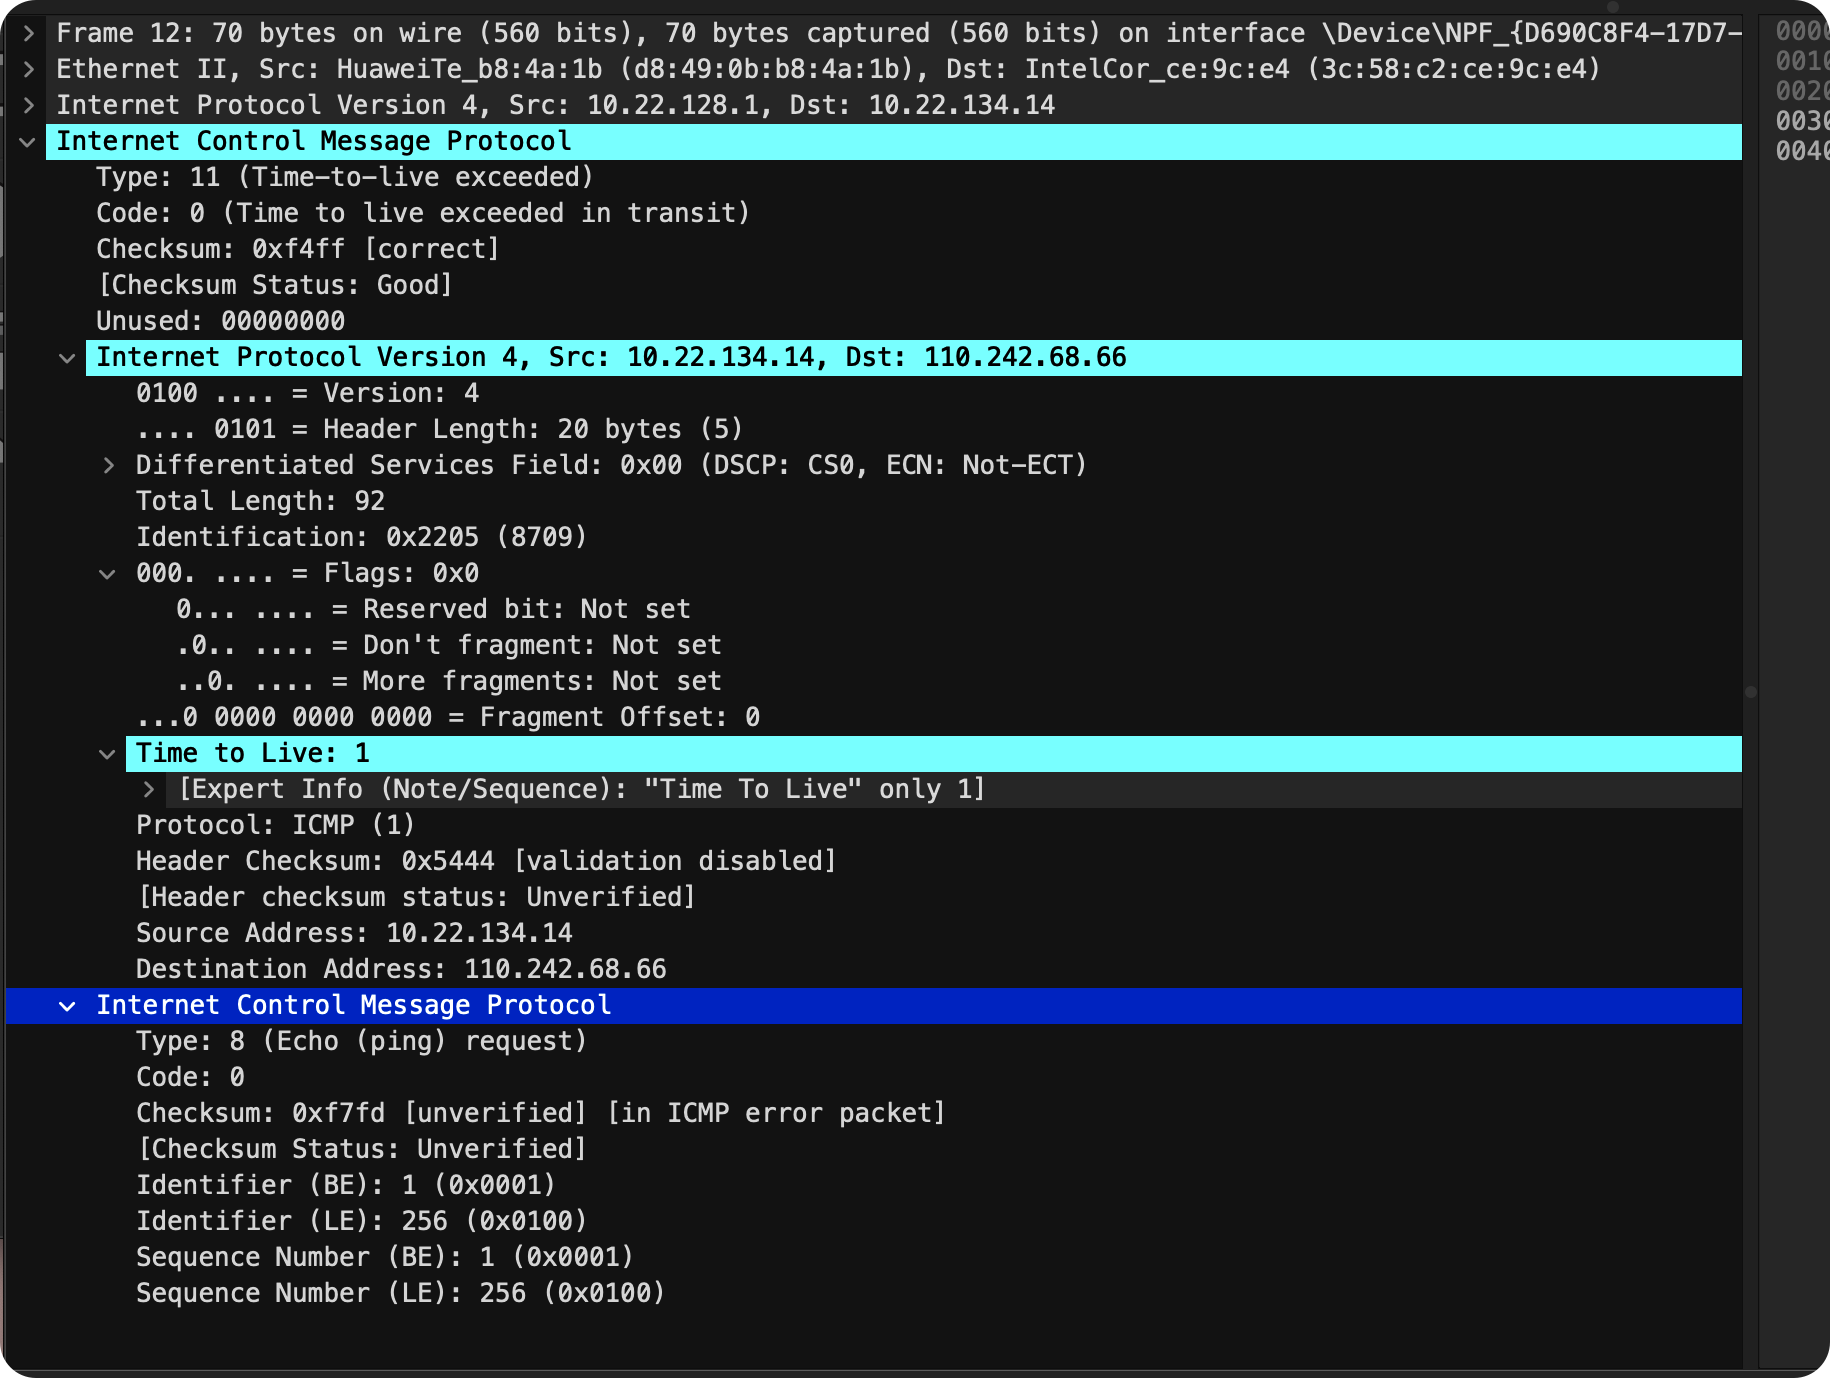
\includegraphics[width=10cm]{figure/ttl.png}
\caption{[ICMP time exceeded] 超时类ICMP差错报文}
\label{pic:ttl}
\end{figure}

tracert命令执行时,源主机发起一个TTL=1的ICMP 报文。第一个路由器收到该报文后,TTL减 1 变为 0 并丢弃此报文,返回一个如图\ref{pic:ttl}的 [ICMP time exceeded] 消息。源主机通过这个消息获知IP数据报转发路径上的第一个路由器信息。

从图\ref{pic:ttl}中我们可以看出,超时类的差错报文Type为11,Code为0。其结构为:类型为11;Code代码为0;校验和未使用(全为0);

除了该差错ICMP自己的信息外,该ICMP还携带了所被丢弃的ICMP报文中的IP数据报首部以及数据的前八个字节,而被丢弃的ICMP数据包中的IP数据报数据为ICMP Rcho request,于是该差错ICMP出现了2个ICMP包头信息,简称ICMP双头包。

我们可以去查询该ICMP差错回应报文对应的被丢弃的报文内容,也就是上一个ICMP(echo request)的ICMP内容。

\begin{figure}[htb!]
  \centering
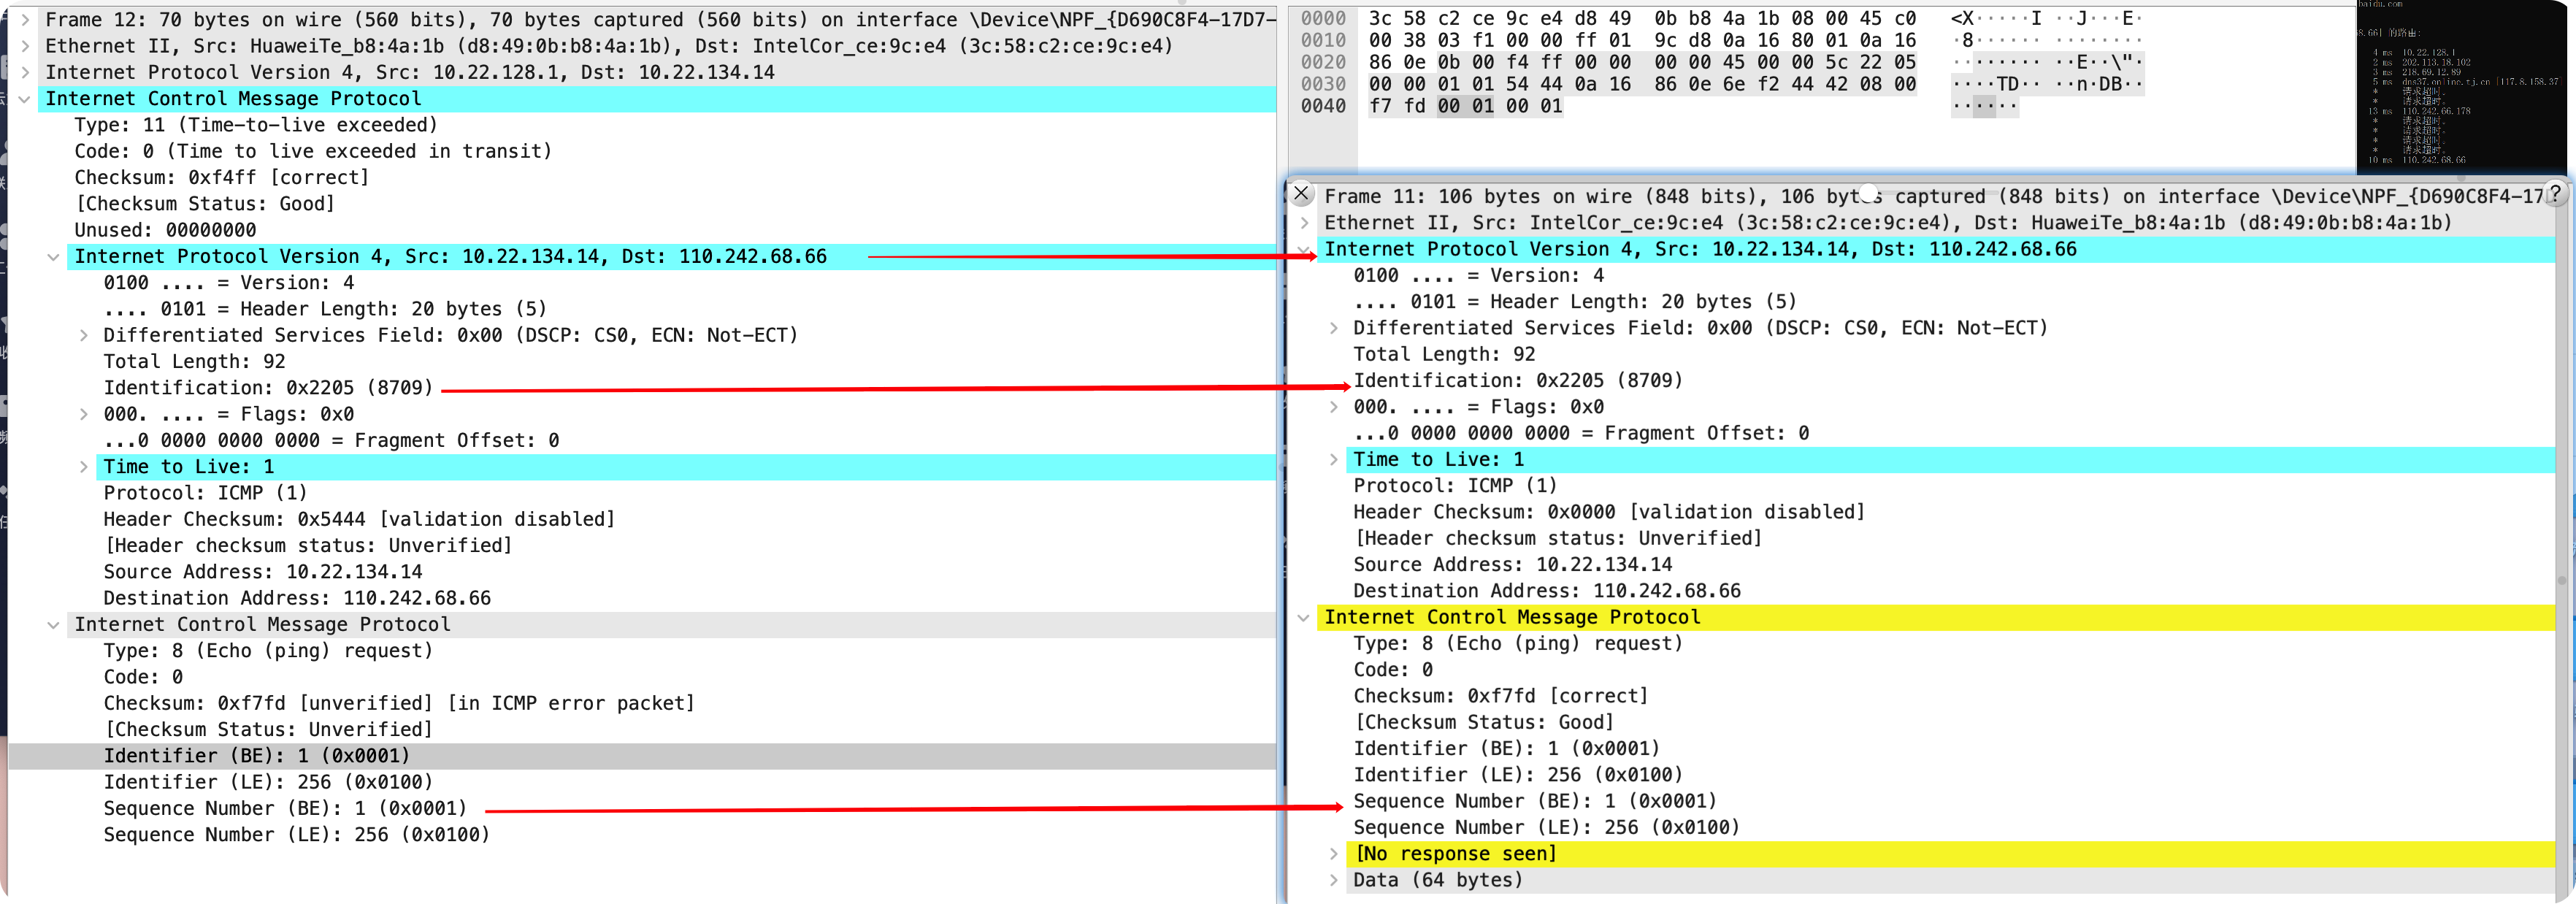
\includegraphics[width=12cm]{figure/timecompare.png}
\caption{ICMP差错报文中含有被丢弃的ICMP echo request报文}
\label{pic:timecompare}
\end{figure}

如图\ref{pic:timecompare},我们可以看到,ICMP差错报文中含有被丢弃的ICMP echo request报文,这个报文的TTL为1,也就是说,这个ICMP差错报文是由第一个路由器返回的。

\begin{figure}[htb!]
  \centering
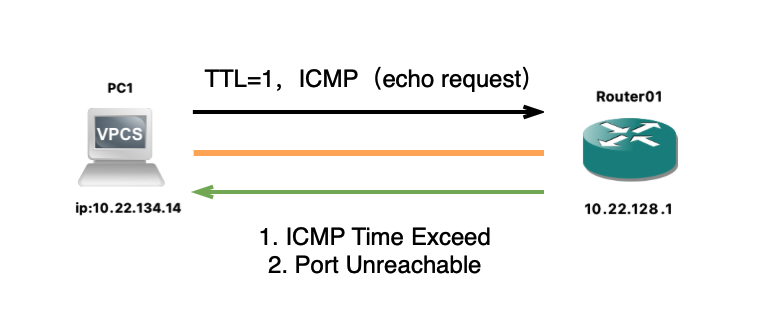
\includegraphics[width=12cm]{figure/ttl-1.png}
\caption{TTL=1的ICMP echo request报文与ICMP差错报文}
\label{pic:ttl-1}
\end{figure}

如图\ref{pic:ttl-1},是第一个路由器响应的完成过程


\paragraph*{[ICMP port unreachable] 端口不可达类ICMP差错报文}


\begin{figure}[htb!]
  \centering
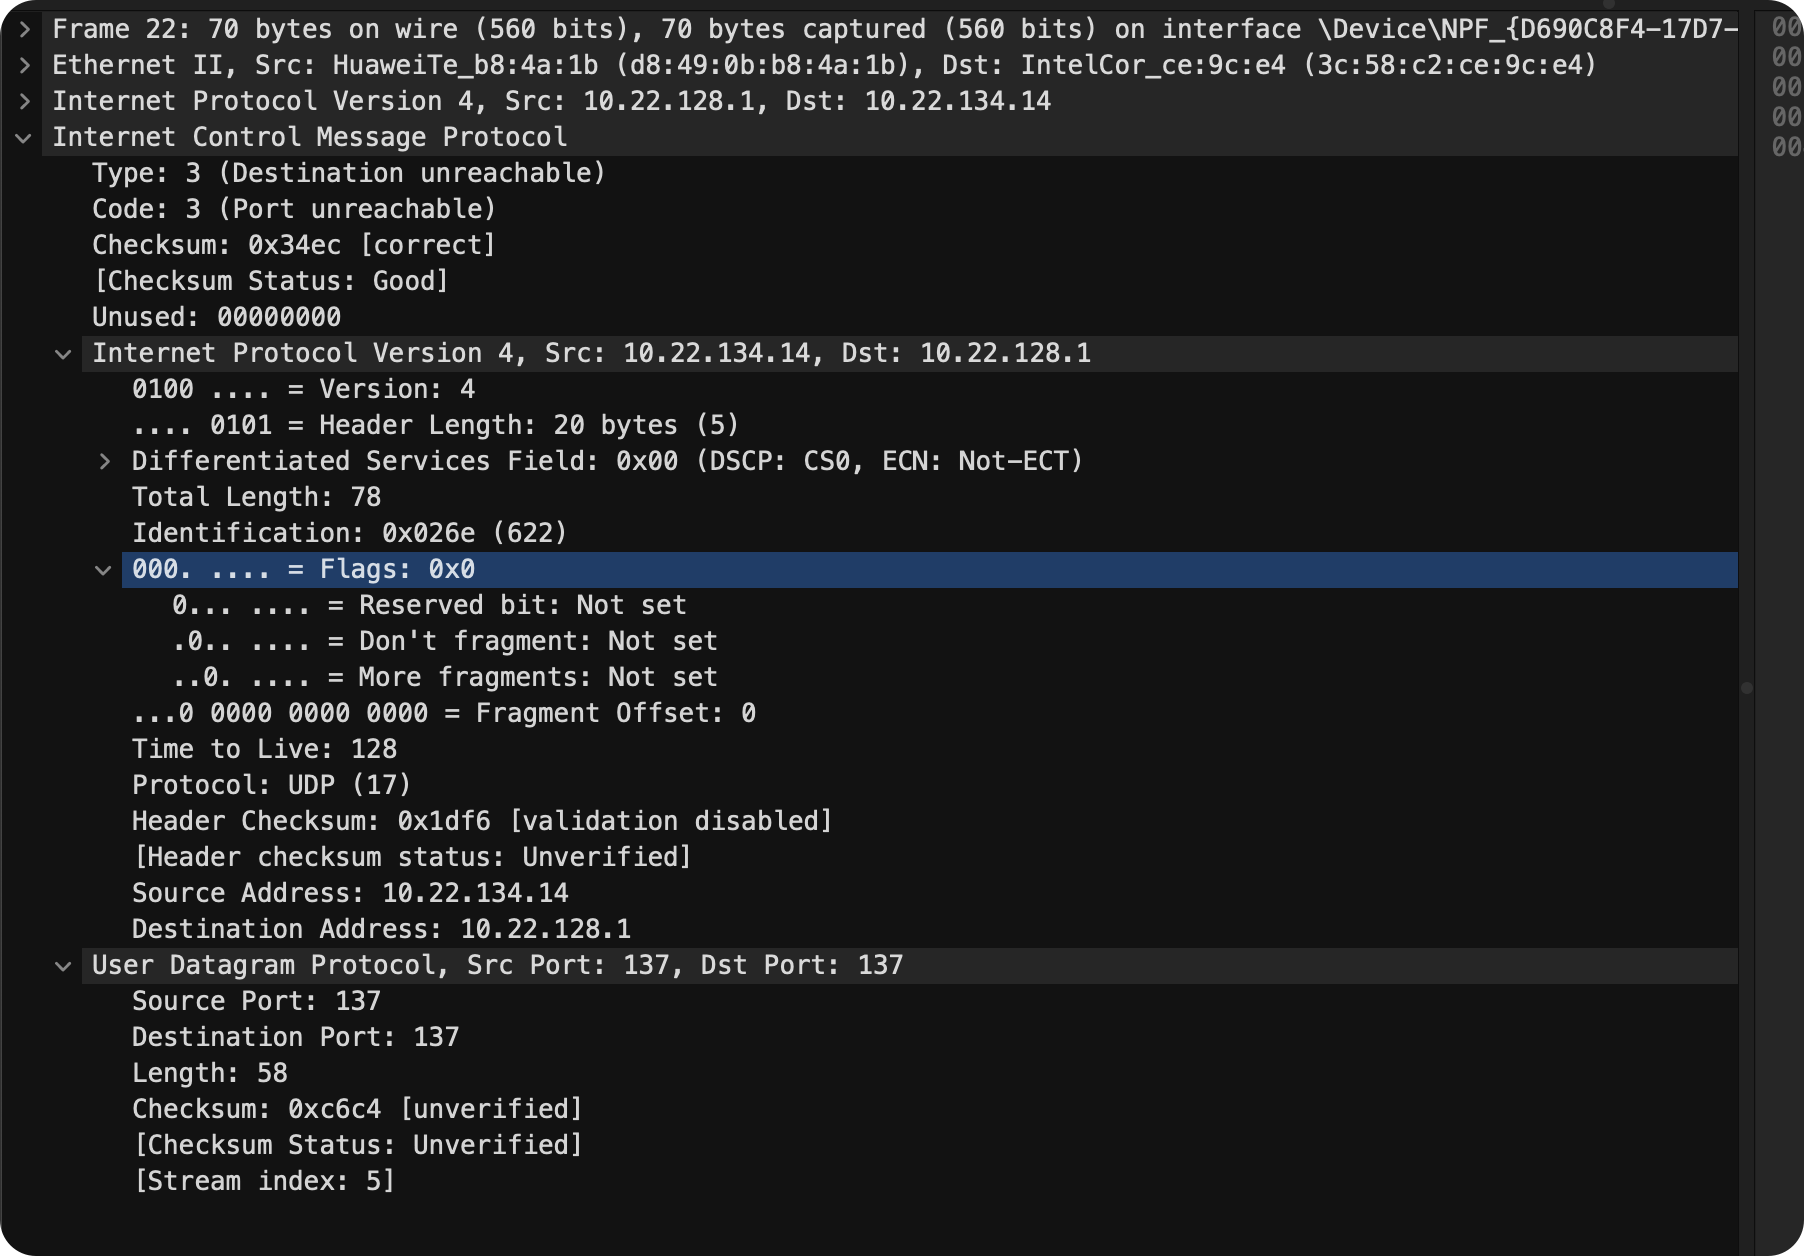
\includegraphics[width=10cm]{figure/des.png}
\caption{[ICMP port unreachable] 端口不可达类ICMP差错报文}
\label{pic:des}
\end{figure}


如图\ref{pic:des},第一个路由器还给我们返回了端口不可达类ICMP差错报文。这个差错报文的Type为3,Code为3。其结构为:类型为3;Code代码为3;校验和未使用(全为0);

那么第一个路由器在丢弃了我发起的TTL=1的ICMP Echo Request报文并返回一个超时类ICMP差错报文后,为什么又返回了一个端口不可达类ICMP差错报文呢? 

\begin{figure}[htb!]
  \centering
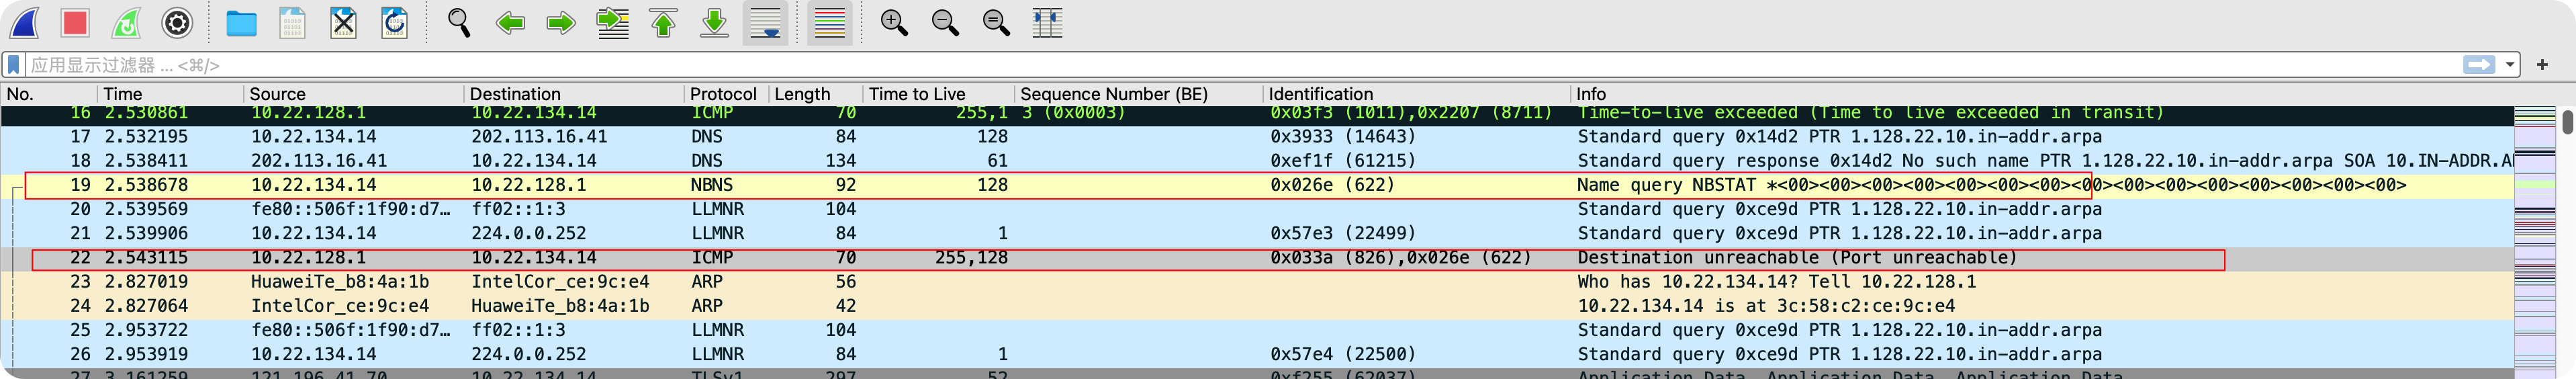
\includegraphics[width=10cm]{figure/nbns.png}
\caption{出现端口不可达类ICMP差错报文的原因}
\label{pic:nbns}
\end{figure}

查看wireshark抓取的数据包,如图\ref{pic:nbns},可以发现我的PC还对第一个路由器发起了一个携带UDP数据报的NBNS协议,从而第一个路由器才又返回了一个端口不可达类ICMP差错报文。

NBNS是NetBIOS name service的缩写,是NetBIOS的命名服务,用于将NetBIOS名称映射到IP地址上,是NetBIOS-over-TCP(NBT)协议族的一份子。NBNS是动态DNS的一种,Microsoft的NBNS实现称为WINS。路由器可以通过发送NBNS状态请求以获取设备名,windows PC 接收到后通过WINS或将本地缓存发送命名信息给路由器。

之所以出现这个端口不可达的ICMP差错报文,是因为该NBNS数据包还没到传输层(UDP$\backslash$TCP)就挂了,网络层看到没有进程在监听指定的协议端口即对端主机没有进程监听的对应请求端口,那么就会通过 ICMP 协议以端口不可达的原因告知主机。

在目标端口不可达的情况下, 就会送回一个“目标端口不可达”的ICMP报文。该错误报文中会包括前8个字节的原数据包内容,这就是你在ICMP中看到的UDP部分,如图\ref{pic:nbns-com}所示。

\begin{figure}[htb!]
  \centering
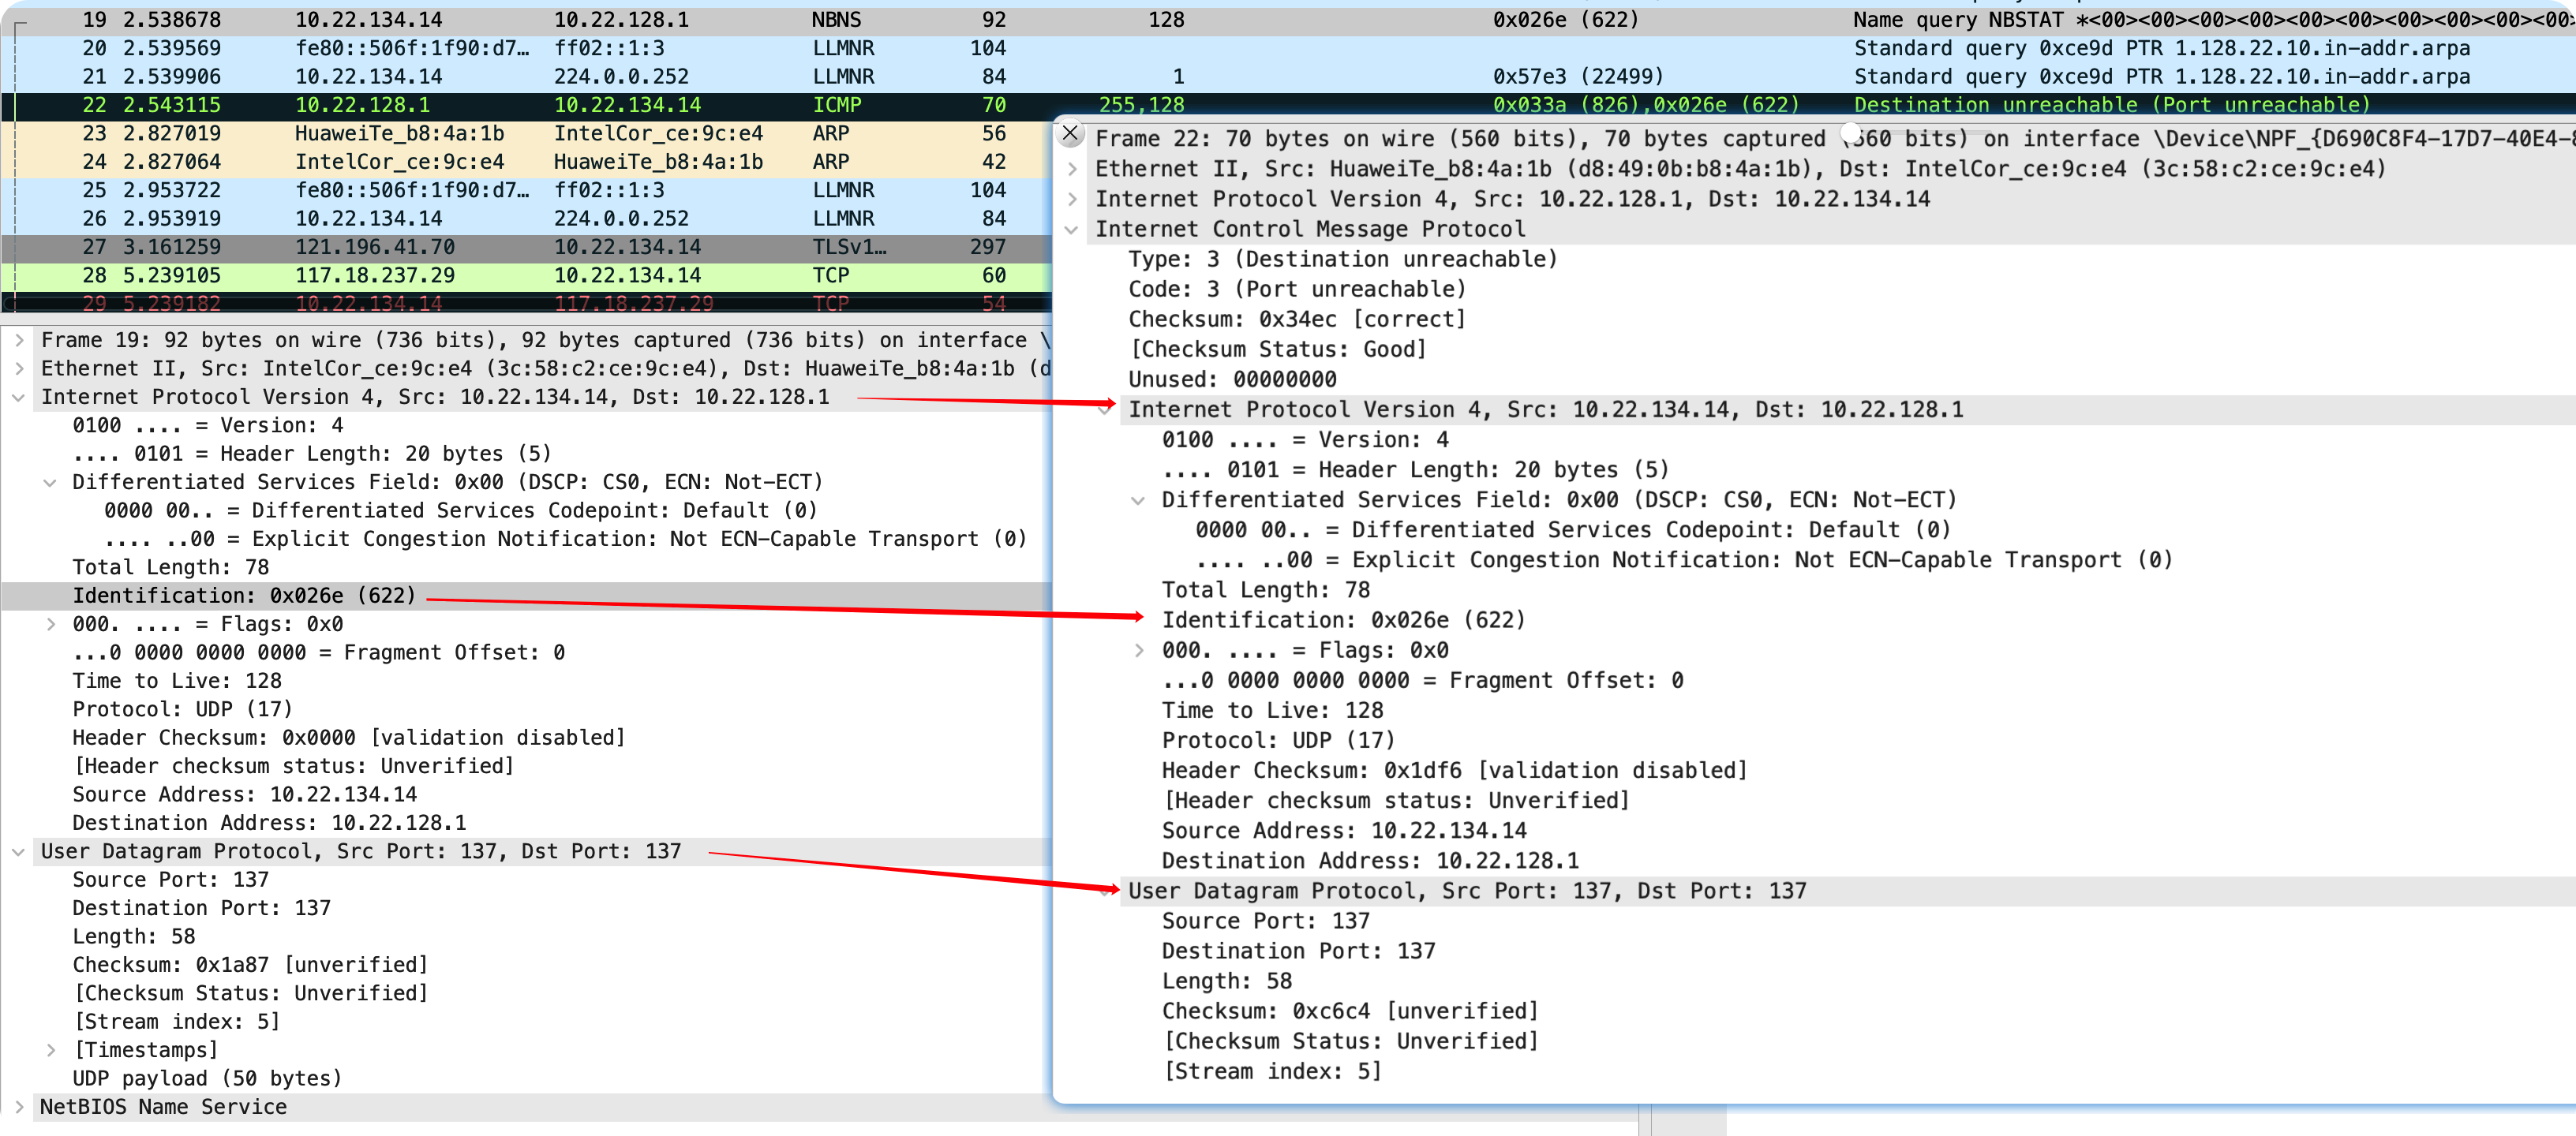
\includegraphics[width=10cm]{figure/nbns-com.png}
\caption{Frame19 NBNS与Frame 22的端口不可达ICMP差错报文}
\label{pic:nbns-com}
\end{figure}

除了在windows系统中,tracert命令执行的过程中会收到这种差错报文,
在MacOS与Linux系统中,Linux和Mac OS使用UDP包进行traceroute探测,目标端口号默认为33434,每次探测目标端口号加1。
Traceroute故意使用了一个大于 30000 的目标端口号,以保证目标地址收到数据包后能够返回一个“端口不可达”的 ICMP 报文,于是源地址就可将端口不可达报文当作跟踪结束的标志。

但是当然,端口不可达类ICMP差错报文不止在跟踪结束时出现,还会在上述这种情况出现,会导致跟踪结果不准确,至少我在使用MacOS抓取了60000多条信息后依然没有得到正确的跟踪结束信息。


\subsubsection{数据交互示意图}
结合我Tracert www.baidu.com得到的图\ref{pic:tracertbaidu}以及使用wireshark抓取的 ICMP 报文记录,
如图\ref{pic:allrouter}是根据Tracert命令可知的信息所有经过的路由器,再根据此,画出数据交互示意图,如图\ref{pic:ttl1}图,\ref{pic:ttl2},图\ref{pic:ttl3},图\ref{pic:ttl4},图\ref{pic:ttl6},图\ref{pic:ttl12},我分别绘制了TTL=1,2,3,4,6,12时的数据交互示意图。

其中TTL=1遇到的第一个路由器以及TTL=3遇到的第三个路由器都因为NBNS协议发出了Port Unreachable的端口不可达ICMP数据报;

在TTL=5,6,8,9,10,11时遇到请求超时的情况;

在TTL=12时遇到了目标主机,得到了目标主机的ICMP Echo Reply回应。

\begin{figure}[htb!]
  \centering
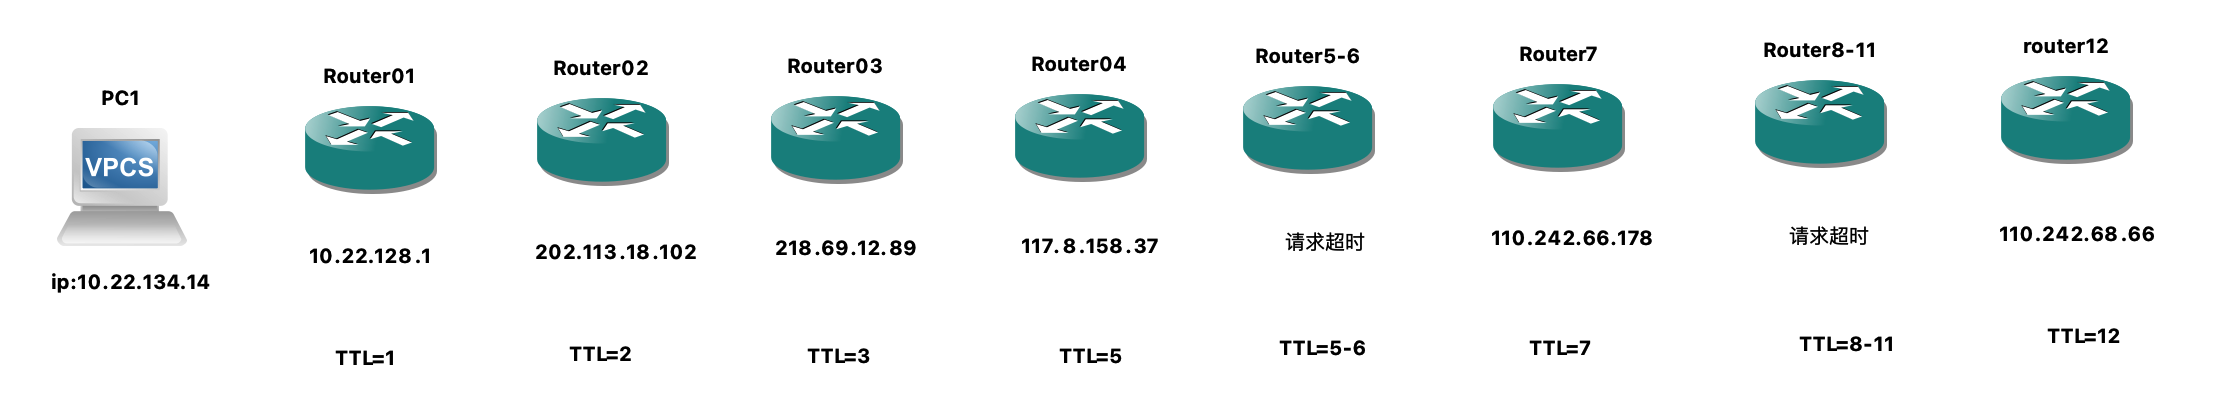
\includegraphics[width=18cm]{figure/allrouter.png}
\caption{信息到达百度服务器所有经过的路由器}
\label{pic:allrouter}
\end{figure}


\begin{figure}[htb!]
  \centering
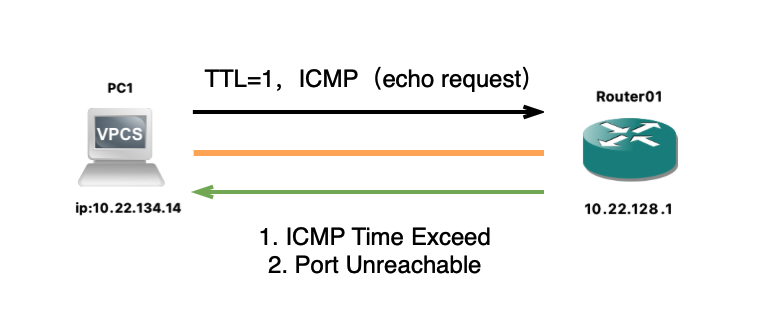
\includegraphics[width=10cm]{figure/ttl-1.png}
\caption{TTL=1时的数据交互示意图}
\label{pic:ttl1}
\end{figure}

\begin{figure}[htb!]
  \centering
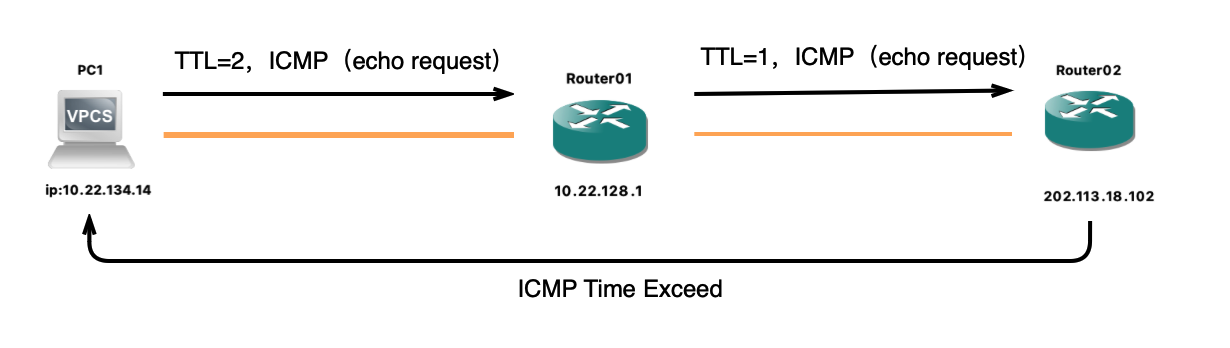
\includegraphics[width=16cm]{figure/ttl-2.png}
\caption{TTL=2时的数据交互示意图}
\label{pic:ttl2}
\end{figure}

\begin{figure}[htb!]
  \centering
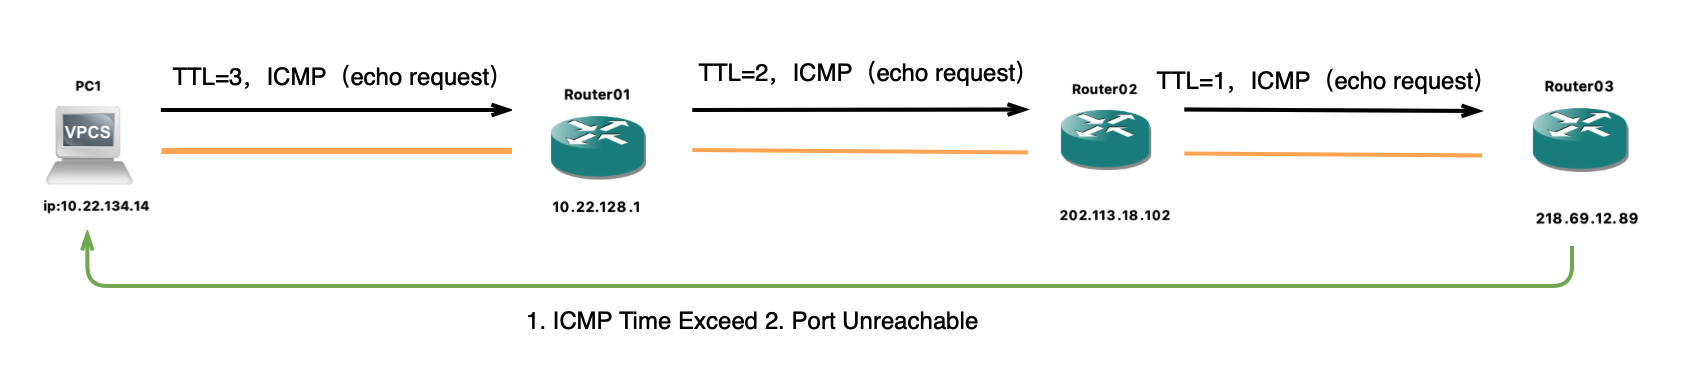
\includegraphics[width=16cm]{figure/ttl-3.png}
\caption{TTL=3时的数据交互示意图}
\label{pic:ttl3}
\end{figure}

\begin{figure}[htb!]
  \centering
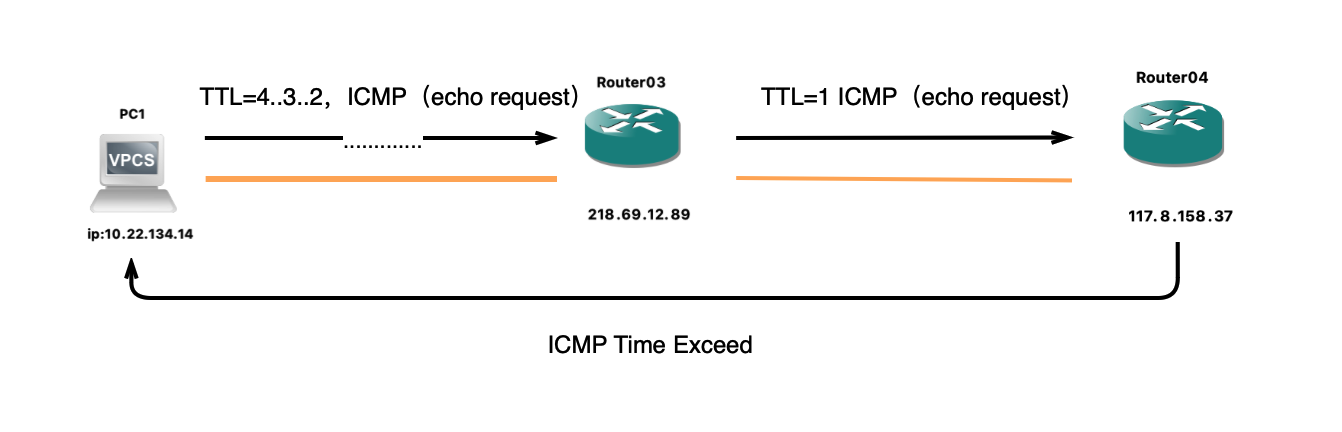
\includegraphics[width=16cm]{figure/ttl-4.png}
\caption{TTL=4时的数据交互示意图}
\label{pic:ttl4}
\end{figure}

\begin{figure}[htb!]
  \centering
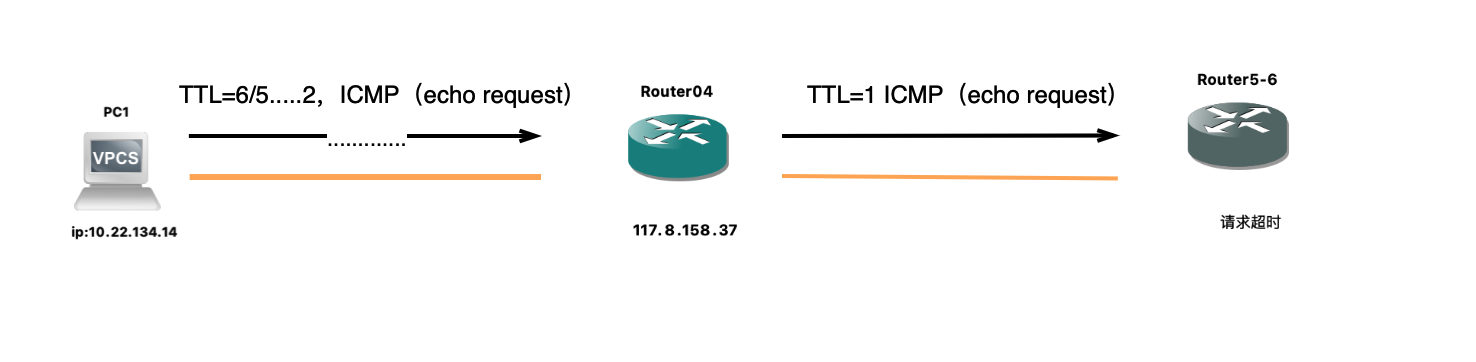
\includegraphics[width=16cm]{figure/ttl-6.png}
\caption{TTL=6时的数据交互示意图}
\label{pic:ttl6}
\end{figure}

\begin{figure}[htb!]
  \centering
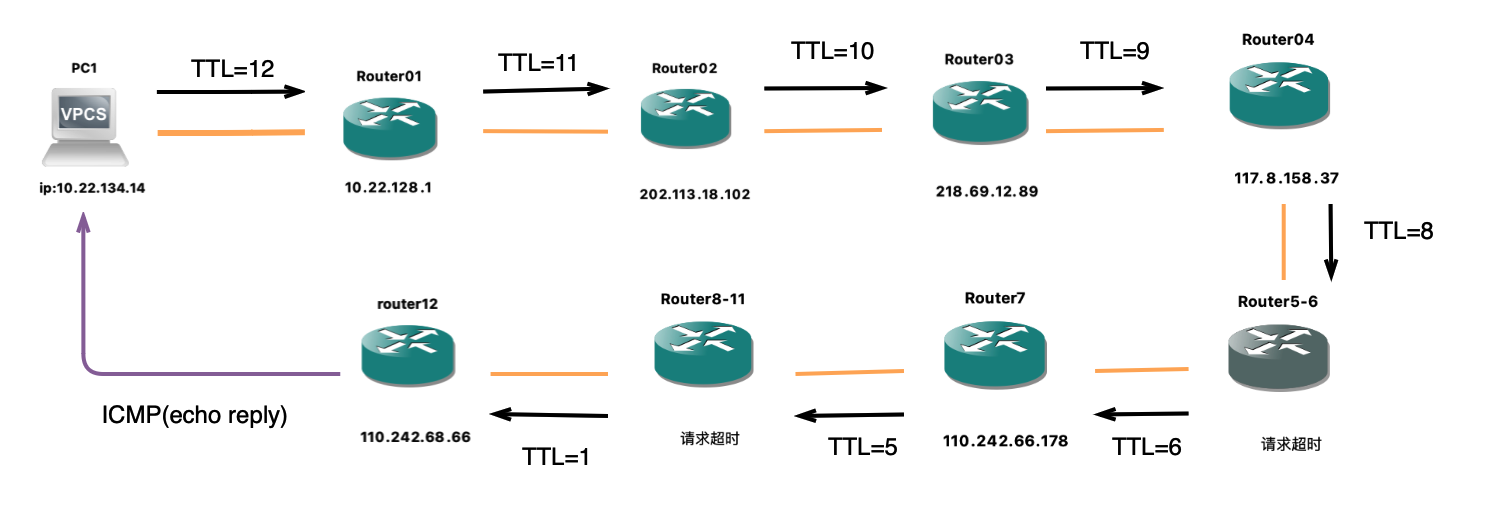
\includegraphics[width=16cm]{figure/ttl-12.png}
\caption{TTL=12时的数据交互示意图}
\label{pic:ttl12}
\end{figure}

% \subsubsection{网关对pc1的arp请求}
% \begin{figure}[h!]
%   \centering
%   \begin{subfigure}[b]{0.3\linewidth}
%     
\includegraphics[width=\linewidth]{figure/nankai.jpg}
%     \caption{观察PC1与Sw3之间.}
%   \end{subfigure}
%   \begin{subfigure}[b]{0.6\linewidth}
%     
\includegraphics[width=\linewidth]{figure/nankai.jpg}
%     \caption{使用WireShark抓取数据包.}
%   \end{subfigure}
%   \caption{使用WireShark抓取PC1与Sw3之间的数据包.}
%   \label{fig:128}
% \end{figure}

\section{实验心得总结}
本次实验观察了IP数据报和ICMP询问报文的结构,
并比较ICMP请求帧与回应帧其IP头部数据字段的异同;
通过改变ping命令的参数,观察IP数据报分片,探索了数据报分片的原因;
了解了Traceroute与Tracert命令的原理,探索了Traceroute与Tracert命令的工作原理;
通过执行Tracert命令,观察ICMP差错报文的结构,并分析其工作原理;
结合捕获的具体数据,绘制了命令执行过程中数据交互的示意图等。
更加深刻地理解了IP数据报和ICMP询问报文的结构和原理,
也理解了通过Tracert命令获取路由信息的过程。

\end{spacing}
\end{document}

%---------------------------------------------------------------------
%  参考文献设置
%---------------------------------------------------------------------
% \addcontentsline{toc}{chapter}{参考文献}

% \begin{thebibliography}{99}
% \songti \zihao{-4} 	
% 	\bibitem{Leslie.{1994}}
% 	Leslie Lamport. LATEX: A Document Preparation System.AddisonWesley, Reading, Massachusetts, second edition, 1994, ISBN 0-201-52983-1.
	
% 	\bibitem{Donald.{1984}}
% 	Donald E. Knuth. The TEXbook, Volume A of Computers and Typesetting,Addison Wesley, Reading, Massachusetts, second edition, 1984,ISBN 0-201-13448-9.

	
% \end{thebibliography}

%---------------------------------------------------------------------
%  附录设置
%---------------------------------------------------------------------
% \titleformat{\chapter}{\heiti\Large}{附录~\Alph{chapter}}{11pt}{\Large}
% \titlespacing{\chapter}{0pt}{*-4}{*4}

% \lstset{breaklines}                %自动将长的代码行换行排版
% \lstset{extendedchars=false}
% \lstset{language=Matlab}
% \renewcommand{\thechapter}{附录\Alph{chapter}.}
% \appendix
% \begin{appendix}
	
	

% \end{appendix}
		


